\documentclass{paper}[11pt]

\usepackage{amsmath, amssymb, mathtools, physics, cleveref, gensymb}
\newcommand{\avg}[1]{\langle{#1}\rangle}
\newcommand{\avgt}[1]{{\avg{\text{#1}}}}
\newcommand{\cnt}[1]{[\text{#1}]}

\newcommand{\arctantwo}{\text{\rmfamily arctan2\normalfont}}
\newcommand{\ut}[1]{{\text{#1}}}
\newcommand{\utx}[2]{{\text{#1}}^{#2}}
\newcommand{\tk}[1]{\ket{\text{#1}}}
\newcommand{\tb}[1]{\bra{\text{#1}}}
\renewcommand{\H}{\tk{H}}
\newcommand{\V}{\tk{V}}
\newcommand{\A}{\tk{A}}
\newcommand{\D}{\tk{D}}
\newcommand{\R}{\tk{R}}
\renewcommand{\L}{\tk{L}}

\newcommand{\HH}{\tk{HH}}
\newcommand{\HV}{\tk{HV}}
\newcommand{\VH}{\tk{VH}}
\newcommand{\VV}{\tk{VV}}

\newcommand{\eHH}{\avgt{HH}}
\newcommand{\eHV}{\avgt{HV}}
\newcommand{\eVH}{\avgt{VH}}
\newcommand{\eVV}{\avgt{VV}}

\newcommand{\HD}{\tk{HD}}
\newcommand{\HA}{\tk{HA}}
\newcommand{\VD}{\tk{VD}}
\newcommand{\VA}{\tk{VA}}

\newcommand{\eHD}{\avgt{HD}}
\newcommand{\eHA}{\avgt{HA}}
\newcommand{\eVD}{\avgt{VD}}
\newcommand{\eVA}{\avgt{VA}}

\newcommand{\eT}{\avgt{T}}

\newcommand{\DR}{\tk{DR}}
\newcommand{\DL}{\tk{DL}}
\newcommand{\AR}{\tk{AR}}
\newcommand{\AL}{\tk{AL}}

\newcommand{\DD}{\tk{DD}}
\newcommand{\DA}{\tk{DA}}
\newcommand{\AD}{\tk{AD}}
\renewcommand{\AA}{\tk{AA}}

\newcommand{\RR}{\tk{DL}}
\newcommand{\RL}{\tk{RL}}
\newcommand{\LR}{\tk{LR}}
\newcommand{\LL}{\tk{LL}}

\newcommand{\eHR}{\avgt{HR}}
\newcommand{\eHL}{\avgt{HL}}
\newcommand{\eVR}{\avgt{VR}}
\newcommand{\eVL}{\avgt{VL}}

\newcommand{\eDD}{\avgt{DD}}
\newcommand{\eDA}{\avgt{DA}}
\newcommand{\eAD}{\avgt{AD}}
\newcommand{\eAA}{\avgt{AA}}

\newcommand{\eDR}{\avgt{DR}}
\newcommand{\eDL}{\avgt{DL}}
\newcommand{\eAR}{\avgt{AR}}
\newcommand{\eAL}{\avgt{AL}}

\newcommand{\eRR}{\avgt{RR}}
\newcommand{\eRL}{\avgt{RL}}
\newcommand{\eLR}{\avgt{LR}}
\newcommand{\eLL}{\avgt{LL}}

\newcommand{\X}{\tk{X}}
\newcommand{\Y}{\tk{Y}}


\newcommand{\HWP}{\text{\rmfamily HWP\normalfont}}
\newcommand{\UVHWP}{\text{\rmfamily UVHWP\normalfont}}
\newcommand{\QWP}{\text{\rmfamily QWP\normalfont}}
\newcommand{\QP}{\text{\rmfamily QP\normalfont}}

\newcommand{\bv}[1]{\textbf{\rmfamily#1\normalfont}}
\newcommand{\xhat}{\hat{\bv{x}}}
\newcommand{\yhat}{\hat{\bv{y}}}
\newcommand{\zhat}{\hat{\bv{z}}}

\newcommand{\BCHWP}{\texttt{B_C_HWP}}
\newcommand{\AHWP}{\texttt{A_HWP}}
\newcommand{\AQWP}{\texttt{A_QWP}}
\newcommand{\BHWP}{\texttt{B_HWP}}
\newcommand{\BQWP}{\texttt{B_QWP}}
\newcommand{\CPCC}{\texttt{C_PCC}}
\newcommand{\CQP}{\texttt{C_QP}}

\newcommand{\pderv}[2]{\frac{\partial{#1}}{\partial{#2}}}
\newcommand{\pdervn}[3]{\frac{\partial^{#3}{#1}}{\partial{#2}^{#3}}}

\renewcommand{\familydefault}{\sfdefault}

\title{How to Calibrate Everything}
\author{Alec Roberson}
\begin{document}
	\maketitle
	\tableofcontents
	
	\section{Jones Matrices and Motor Conventions}
	Unfortunately there are different conventions for how we are defining the ``angle" that each wave plate is rotated to. This means that the Jones matrices defining our optical components will be a little Jenky. In general quantum optics, the convention is that you define $\theta$ as an angle CCW from the horizontal. Using this convention, the Jones matrices for our components are
	\begin{align}
		\QWP &= \begin{pmatrix}
			\cos^2\theta + i\sin^2\theta & \frac{1-i}{2}\sin2\theta \\
			\frac{1-i}{2}\sin2\theta & \sin^2\theta + i\cos^2\theta
		\end{pmatrix} \\
		\HWP &= \begin{pmatrix}
			\cos2\theta & \sin2\theta \\
			\sin2\theta & -\cos2\theta
		\end{pmatrix}
	\end{align}
	Unfortunately, none of our components obey this convention.
	
	\subsection{Elliptec Motors}
	All the Elliptec motors are calibrated so that the ``angle" of the wave plate is defined as an angle CW from the vertical axis. This means that from the original Jones matrices, $\theta\rightarrow\theta'=\frac{\pi}{2}-\theta$. With that, the Elliptec component Jones matrices are
	\begin{align}
		\QWP_E &= \begin{pmatrix}
			\cos^2\theta + i\sin^2\theta & \frac{1-i}{2}\sin2\theta \\
			\frac{1-i}{2}\sin2\theta & \sin^2\theta + i\cos^2\theta
		\end{pmatrix} \\
		\HWP_E &= \begin{pmatrix} -\cos2\theta & \sin2\theta \\ \sin2\theta & \cos2\theta
		\end{pmatrix}
	\end{align}
	
	\subsection{ThorLabs Motors}
	For these measurement components, we define $\theta$ as the CW angle from the horizontal axis. This means we just have to replace $\theta\rightarrow\theta'=-\theta$. The Jones matrices for ThorLabs components then are
	\begin{align}
		\QWP_T &= \begin{pmatrix}
			\cos^2\theta + i\sin^2\theta & \frac{i-1}{2}\sin2\theta \\
			\frac{i-1}{2}\sin2\theta & \sin^2\theta + i\cos^2\theta
		\end{pmatrix} \\
		\HWP_T &= \begin{pmatrix}
			\cos2\theta & -\sin2\theta \\ -\sin2\theta & -\cos2\theta
		\end{pmatrix}
	\end{align}
		
	\section{Homing ThorLabs Motors (Measurement Wave Plates)}
	Using the Kinesis software appears to be able to provide a consistent home position for all of the motors. This home position appears on the dial as somewhere between 8 and 9 degrees for each motor. For completeness, I've included images of each motor in its home position in \cref{fig:AHWP home}-\ref{fig:BQWP home}.
	
	It is a good idea to check in that the motors are homed periodically. You can do this by opening Kinesis, and observing that each motor has a green light next to the word ``homed" in the top right corner. If a motor does not appear, use the ``connect" button in the top left corner of the window.
	
	\subsection{Debugging}
	
	\paragraph{NOTE} the 
	
	\paragraph{DO NOT} press the ``home" button on a motor that has already been homed. This will set the motor's home to be the current position. If you do this, you will need to disconnect from the motor in Kinesis, power cycle the motor manually (unplug it and plug it back in) and then reconnect in Kinesis. At this point, the ``homed" indicator should be orange (and you may even see some extra errors in the log). Now you can hit the ``home" button and 
	
	\begin{figure}[hp]
		\centering
		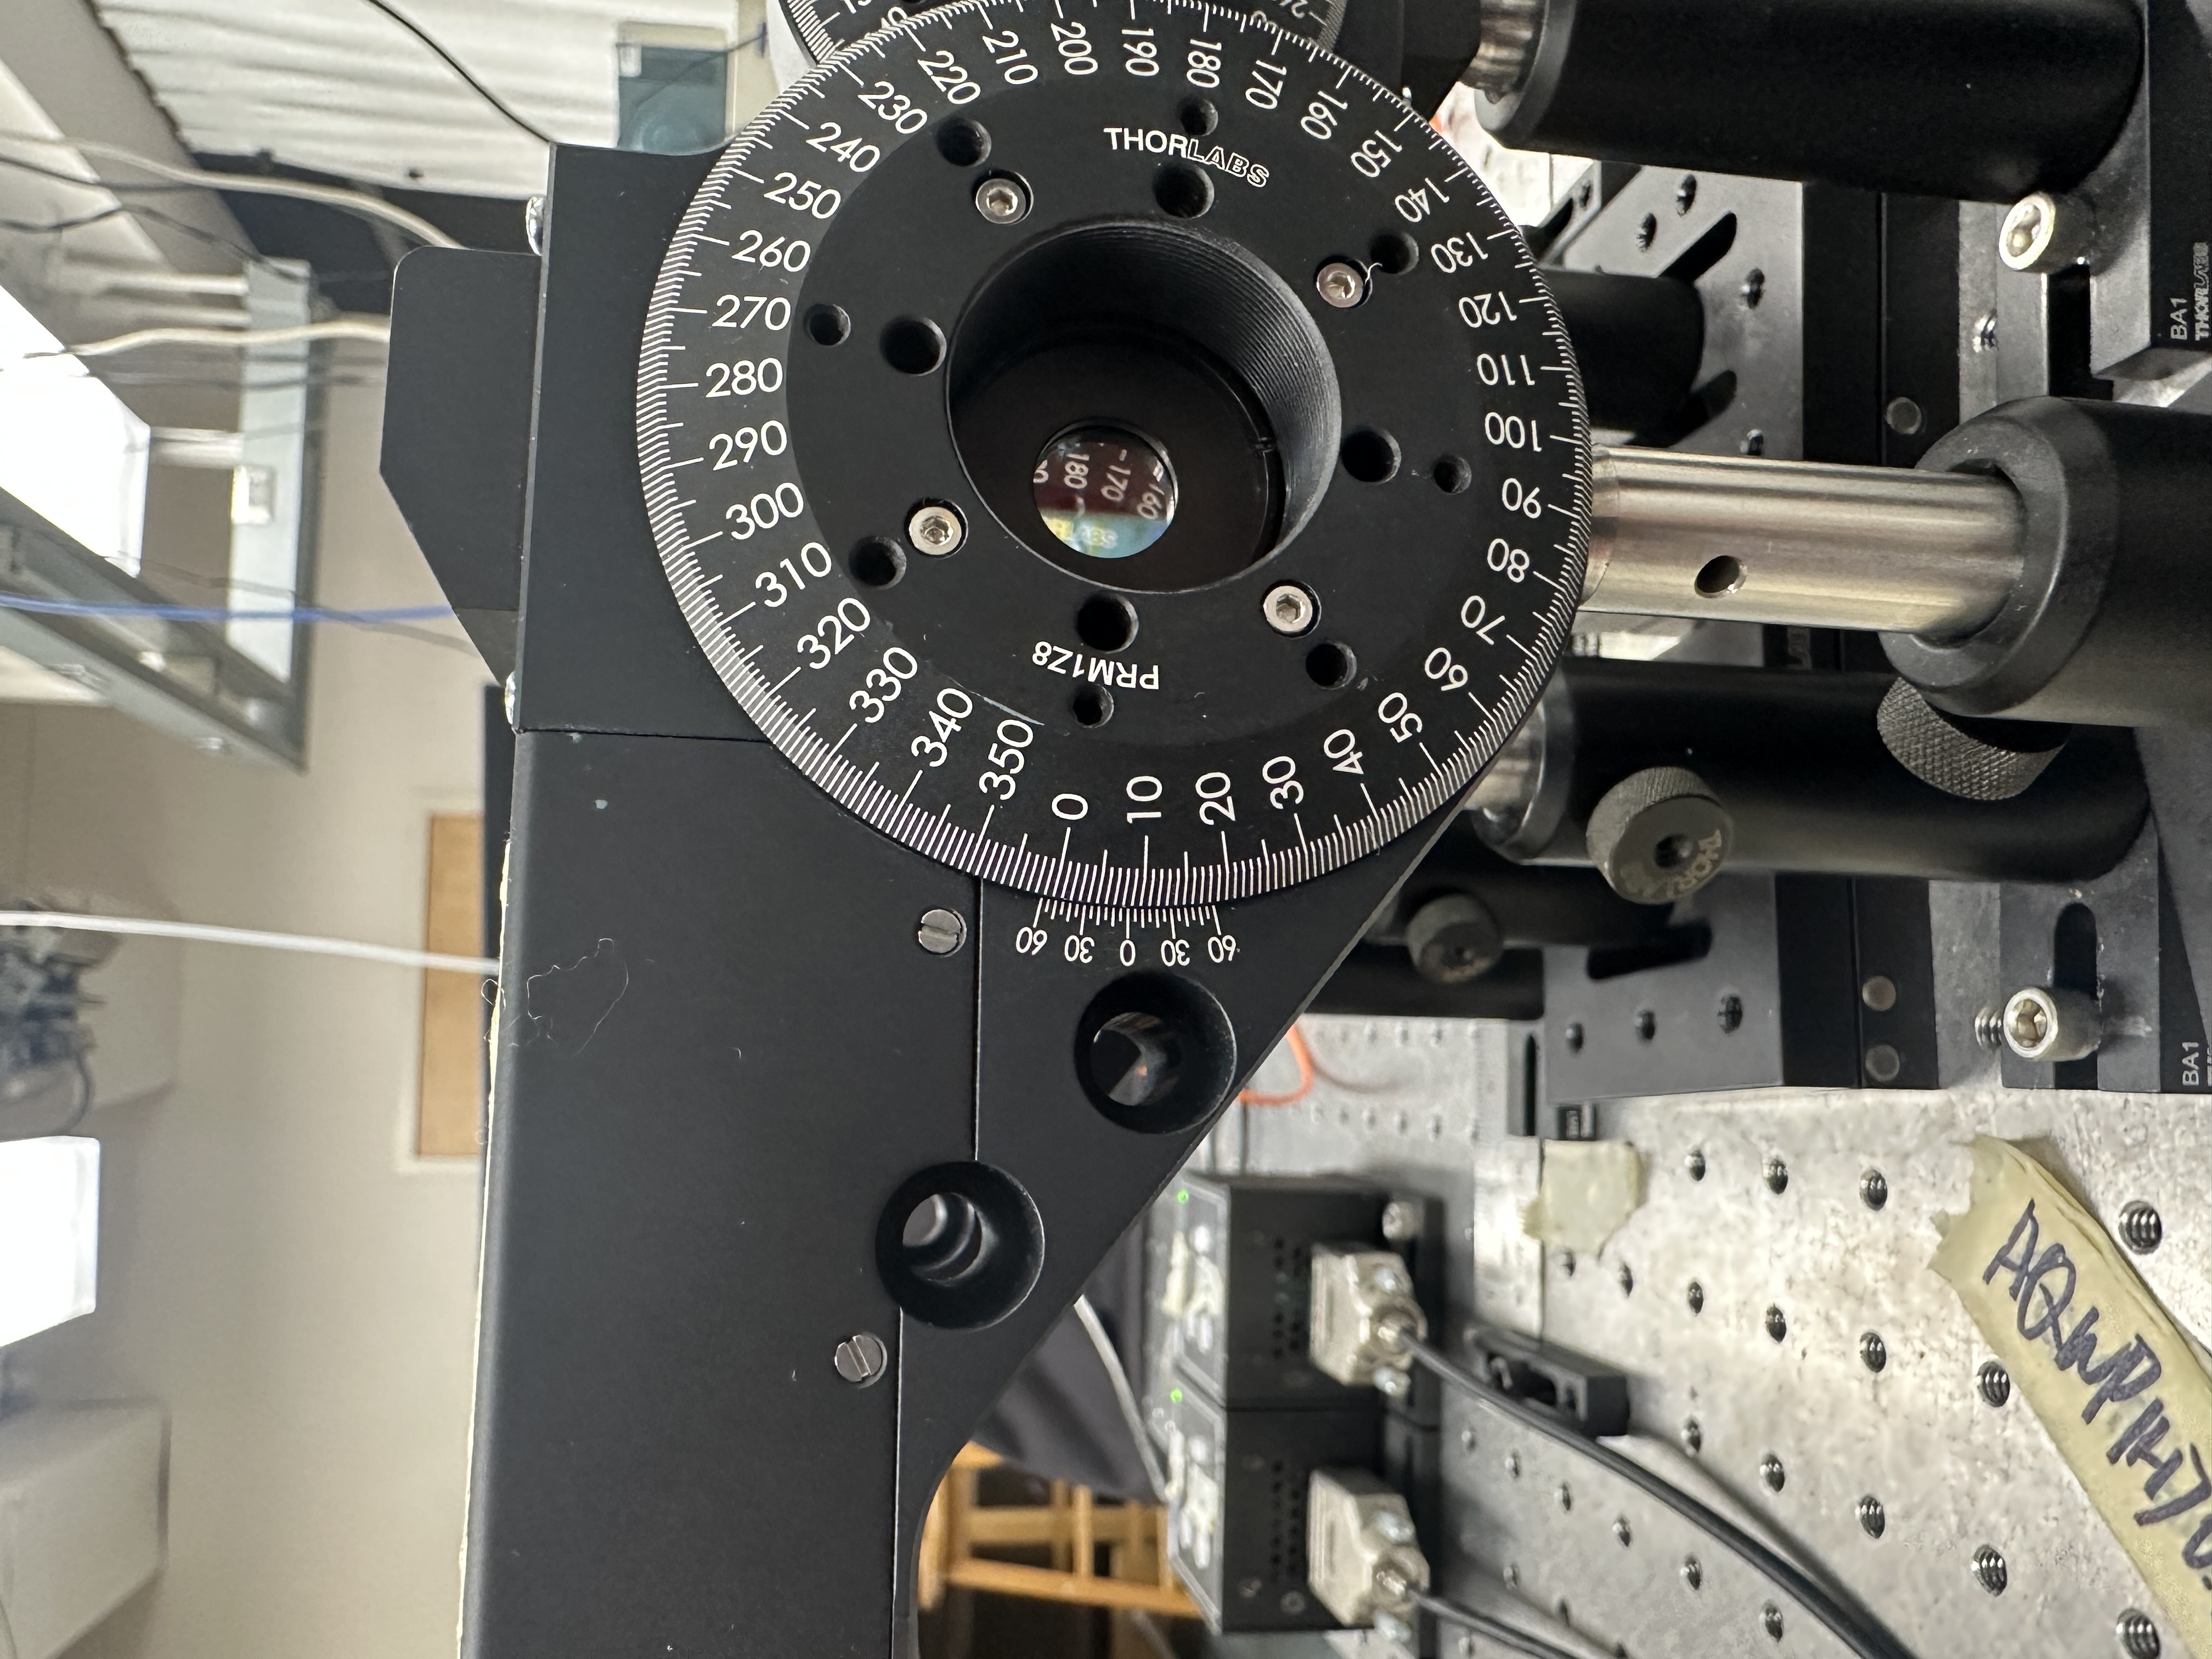
\includegraphics[angle=-90, origin=c, width=0.5\textwidth]{figures/AHWP_HOME.JPG}
		\caption{Alice's half wave plate in its home position.}
		\label{fig:AHWP home}
	\end{figure}
	\begin{figure}[hp]
		\centering
		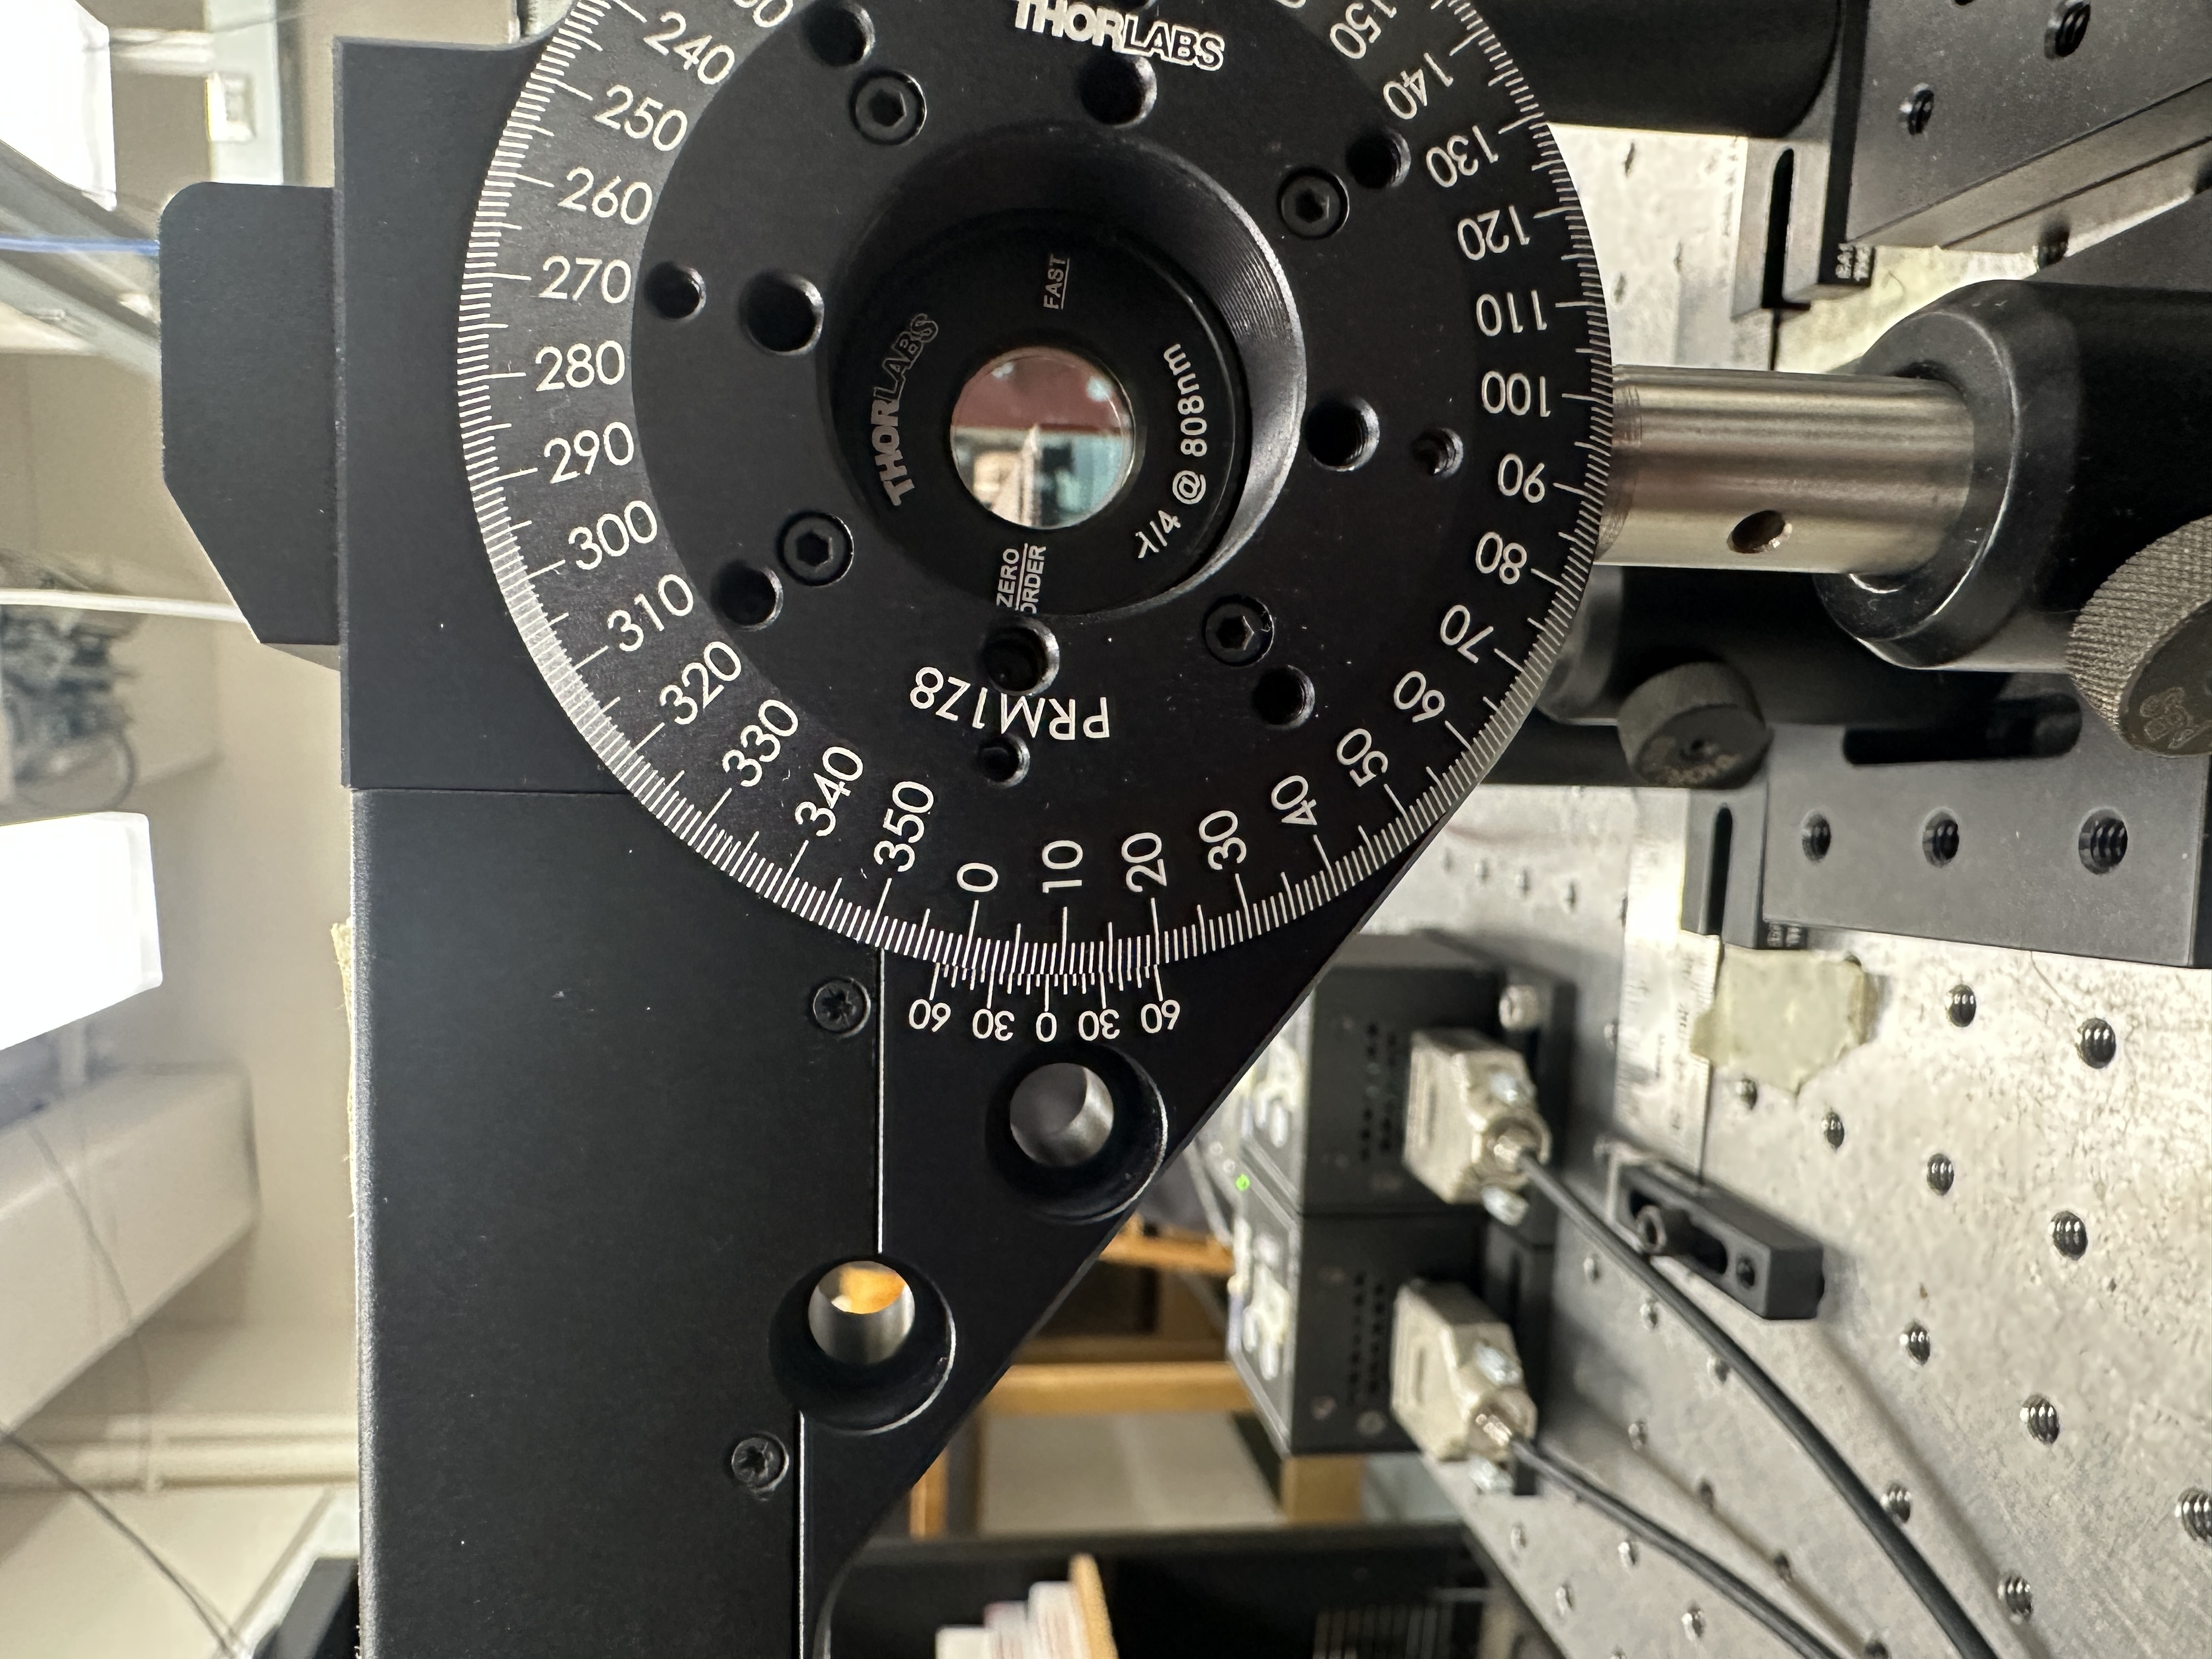
\includegraphics[angle=-90, origin=c, width=0.5\textwidth]{figures/AQWP_HOME.JPG}
		\caption{Alice's quarter wave plate in its home position.}
		\label{fig:AQWP home}
	\end{figure}
	\begin{figure}[hp]
		\centering
		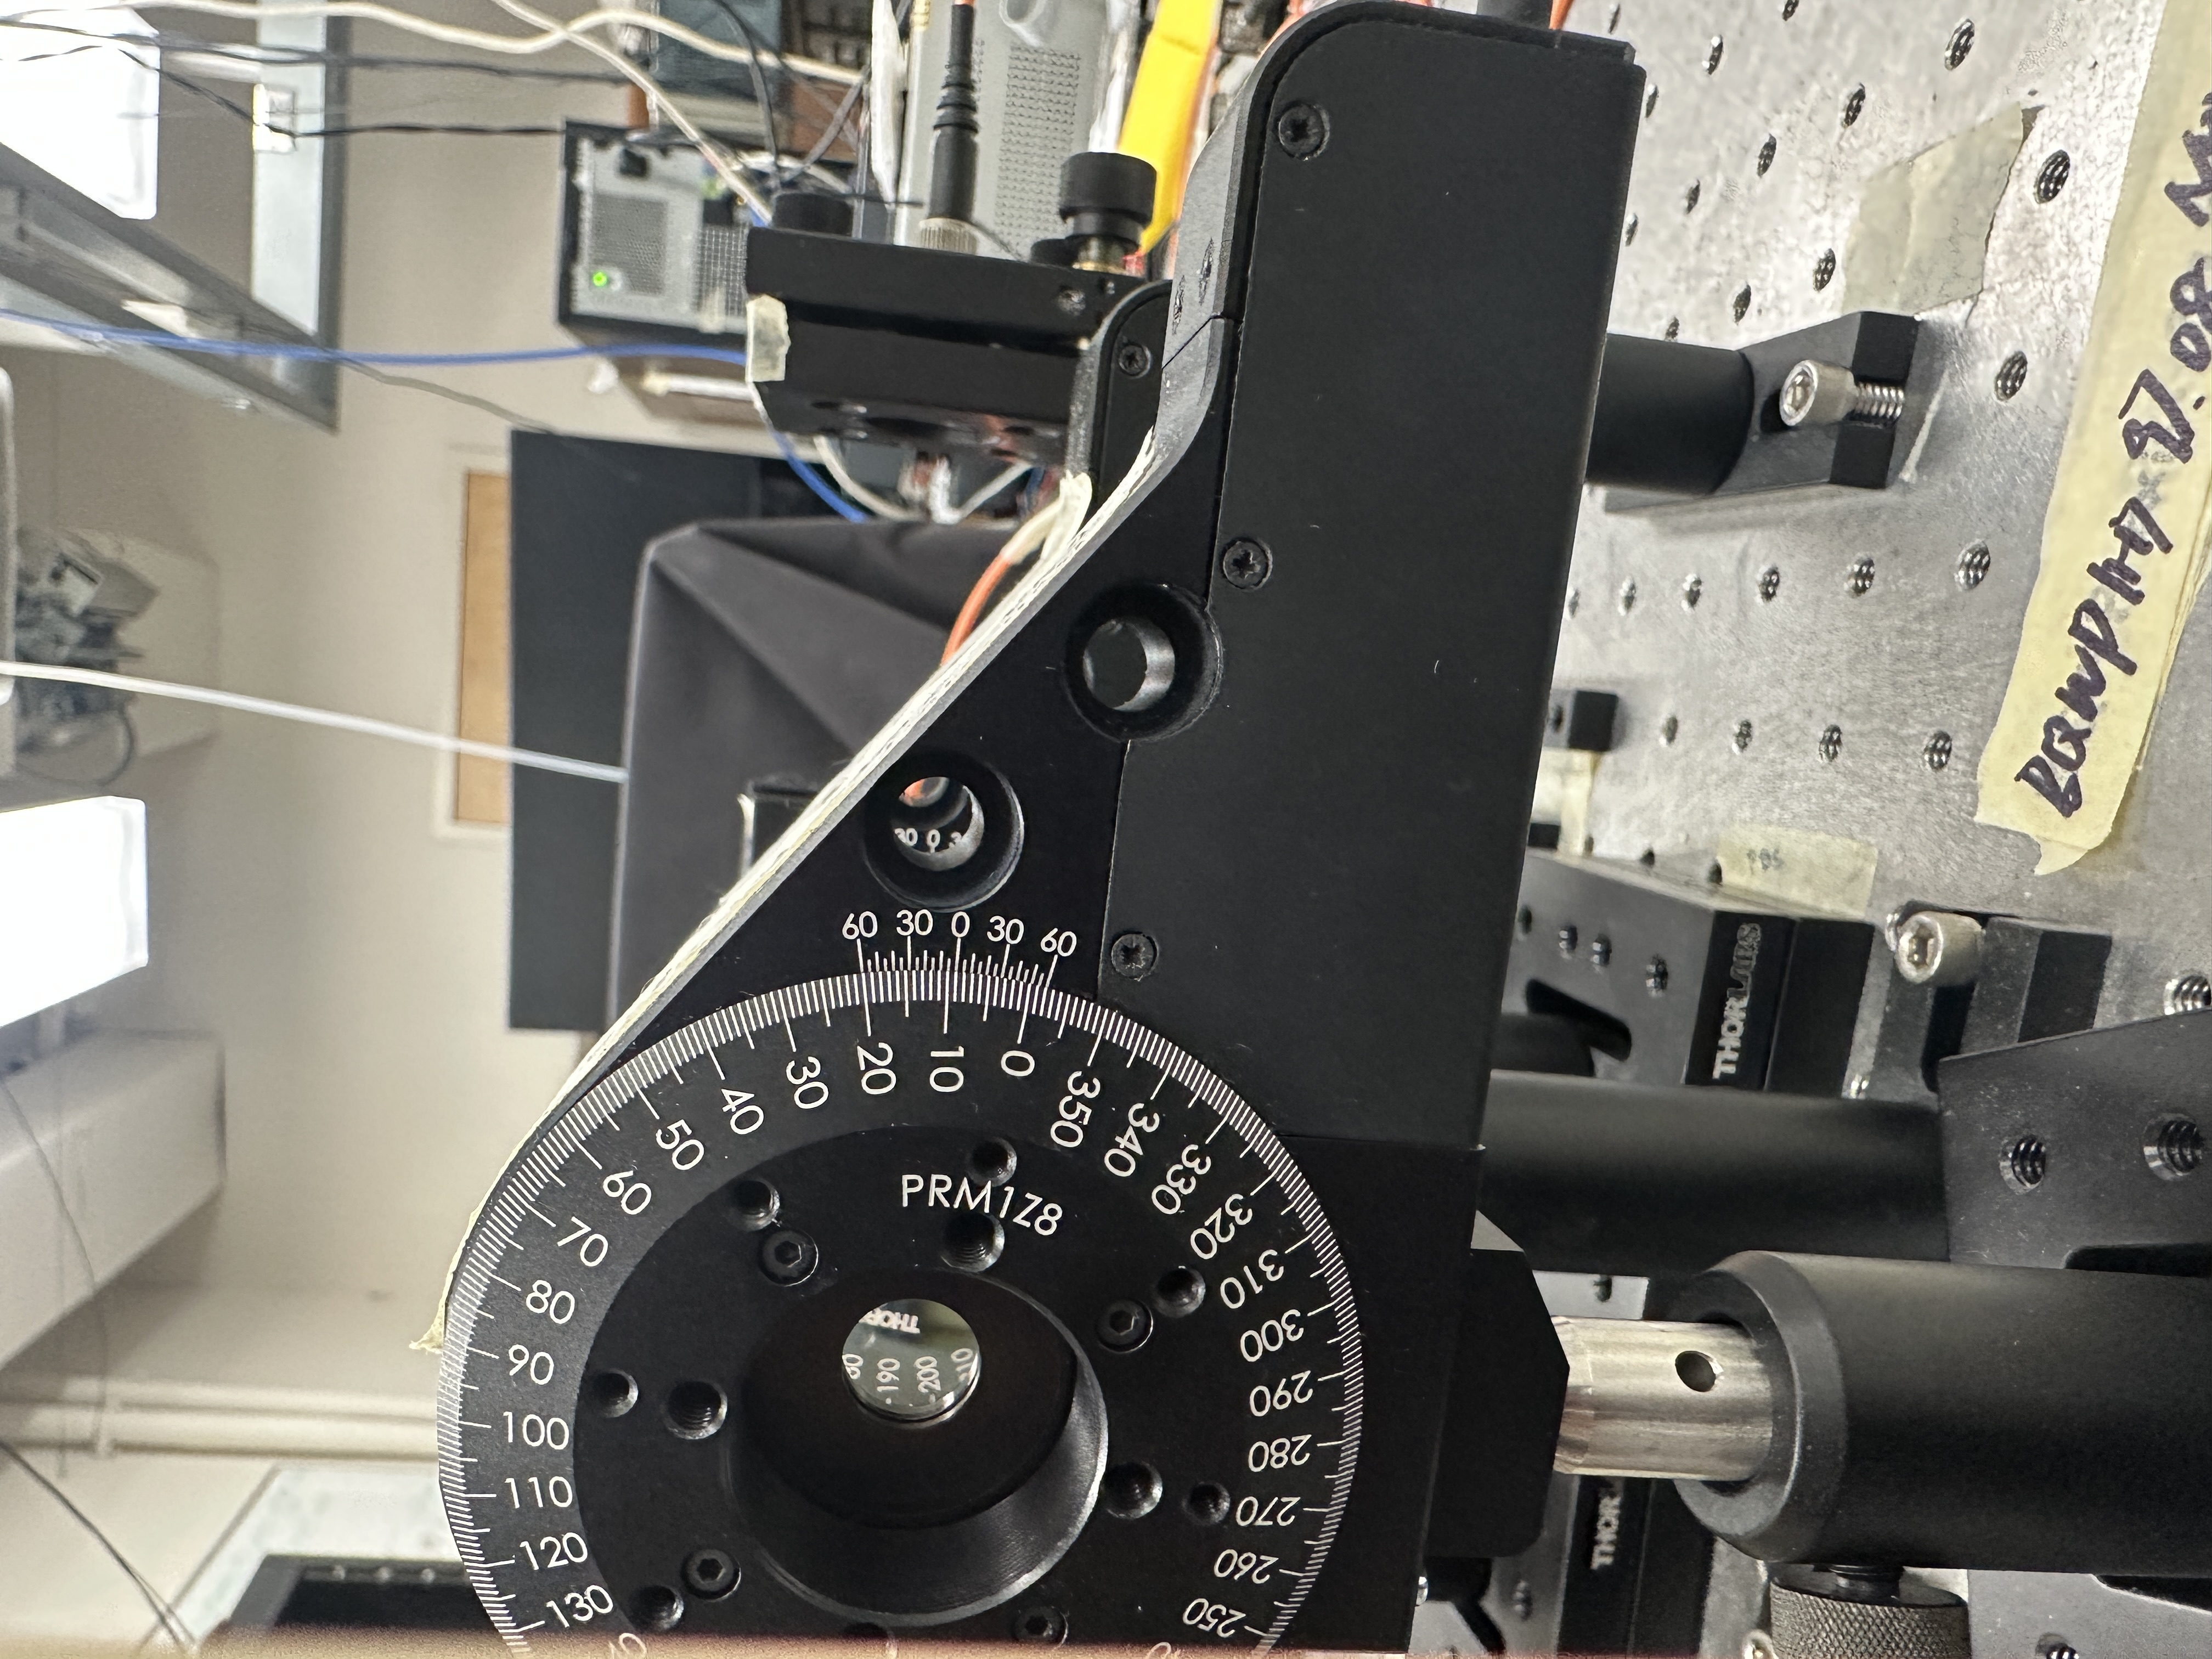
\includegraphics[angle=-90, origin=c, width=0.5\textwidth]{figures/BHWP_HOME.JPG}
		\caption{Bob's half wave plate in its home position.}
		\label{fig:BHWP home}
	\end{figure}
	\begin{figure}[hp]
		\centering
		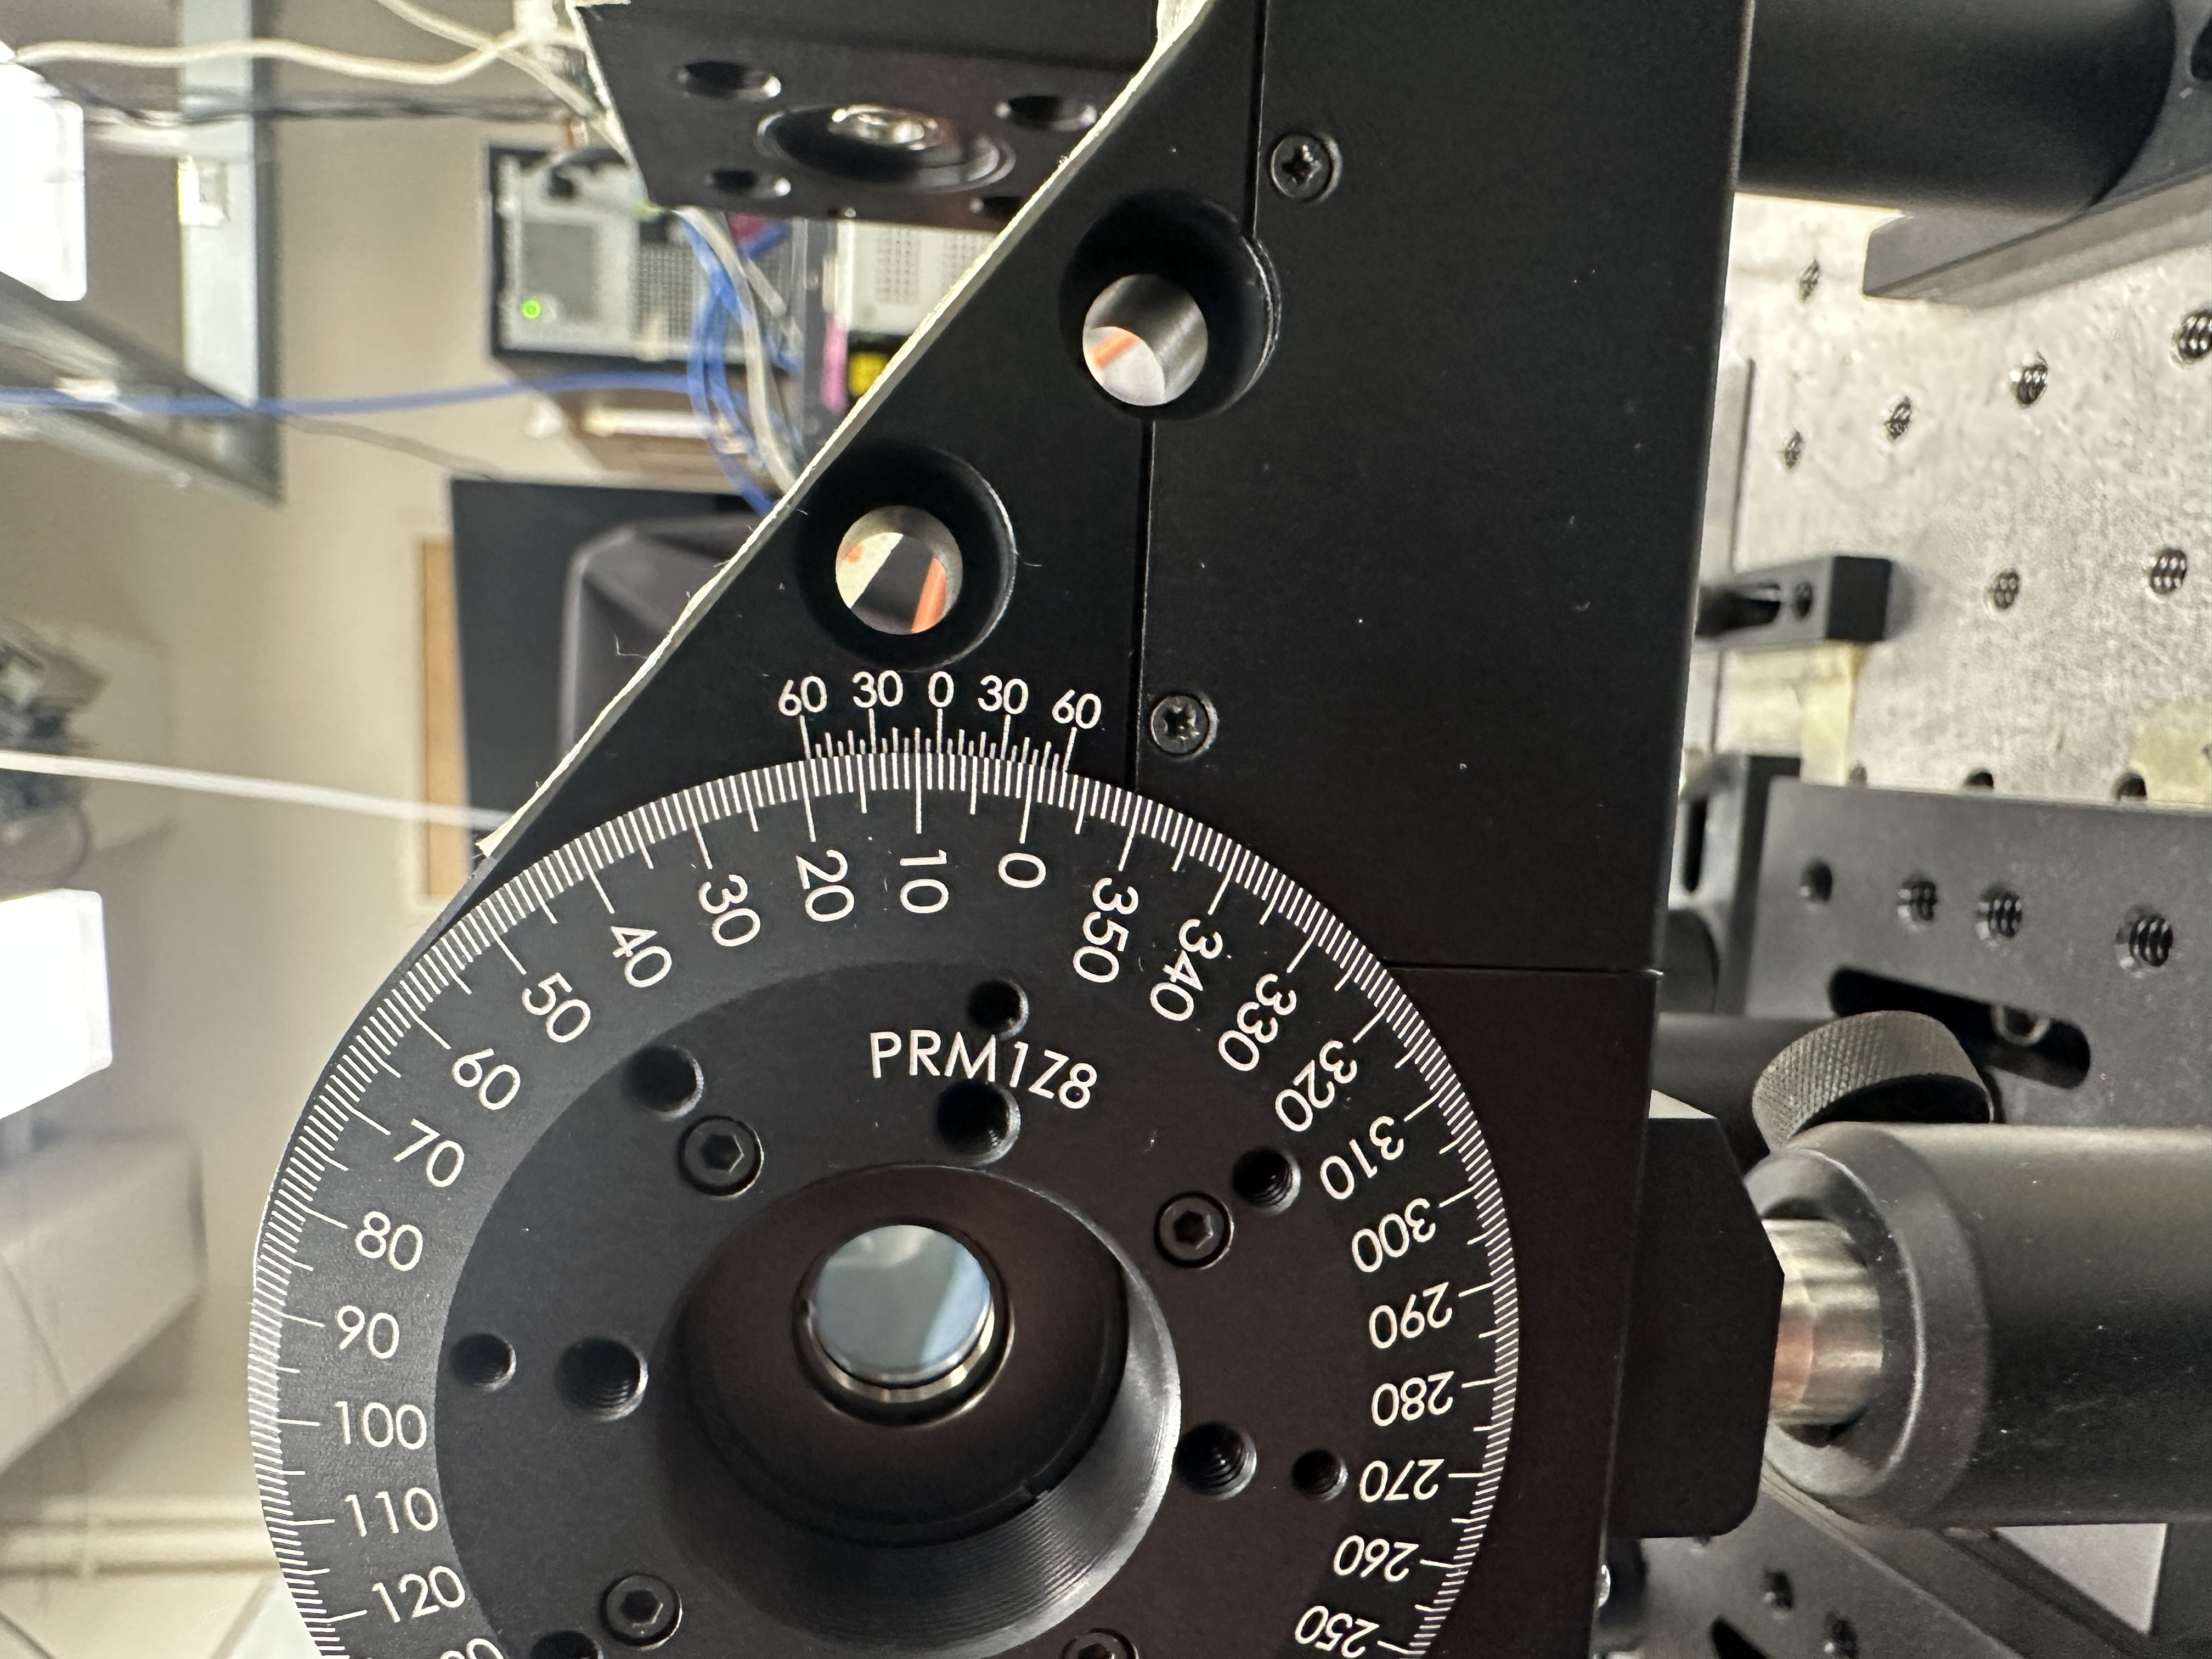
\includegraphics[angle=-90, origin=c, width=0.5\textwidth]{figures/BQWP_HOME.JPG}
		\caption{Bob's quarter wave plate in its home position.}
		\label{fig:BQWP home}
	\end{figure}
	
	\section{A Note on Laser Drift}
	Experiments earlier this summer revealed that our laser experiences some effect that we dubbed ``drift," wherein the angle of the UVHWP that balances HH and VV detections could change by a few degrees as the laser ``warmed up." There is lots of data and explanations about this elsewhere, but the note I want to make here is that this drift will not affect this part of the calibration routine. One of the earliest experiments we did in diagnosing this drift was trying to find the angle of the UV HWP that would minimize VV detections when the laser had just been turned on and when it was warmed up. At the time we suspected the UV HWP's optical properties could be changing throughout the day, over- or under-rotating the light at different temperatures. However, we discovered quite the opposite: separate data taken when the setup either cold or warm (\cref{fig:min VV cold} and \cref{fig:min VV warm}, respectively) show that the angle of the UV HWP that minimizes VV detections did not change beyond its own uncertainty. This seems to indicate that this drift affect is only really notable in situations where the \textit{ratio} between HH and VV detections is what you care about, however at the extrema where you want either only HH or only VV, the lasers ``drift" is negligible.
	
	In calibrating the measurement wave plates I did not really concern myself with the drift during these stages since we were essentially only experimenting with the pure state $\VV$.
	
	\begin{figure}[p]
		\centering
		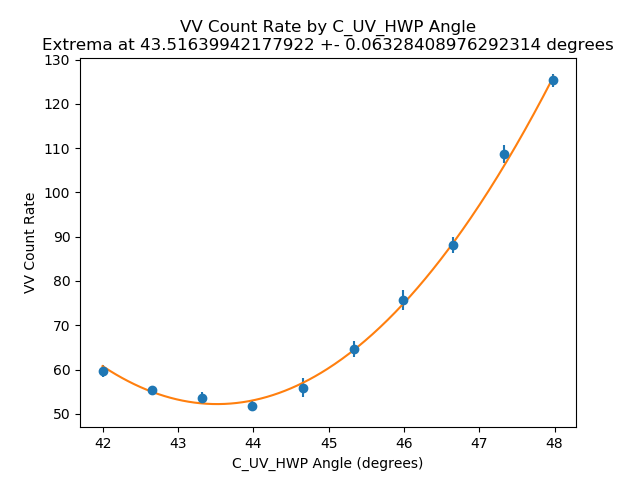
\includegraphics[width=0.8\textwidth]{figures/min_VV_cold.png}
		\caption{VV count rates when the laser had just been switched on (cold).}
		\label{fig:min VV cold}
	\end{figure}
	\begin{figure}[p]
		\centering
		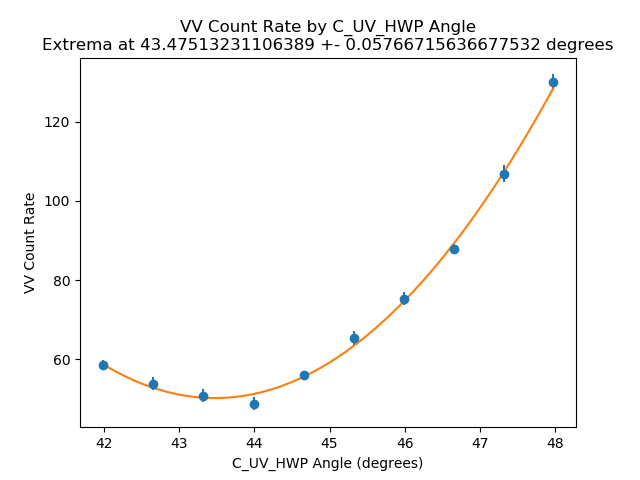
\includegraphics[width=0.8\textwidth]{figures/min_VV_warm.png}
		\caption{VV count rates after the laser had been running up for several hours (warm).}
		\label{fig:min VV warm}
	\end{figure}
	
	\section{Alice's Measurement Wave Plates and the UV HWP}
	
	Unfortunately, on July 14th 2023 Bob's measurement HWP has a USB-protocol error in the middle of a rotation, causing it to lose track of it's home position. Attempts to fix it ended up causing the same error for Bob's measurement QWP and also errors in Alice's measurement wave plates. The point being that now I have to recalibrate this setup from scratch. So here is how I am going to go about that, starting with Alice's measurement wave plates and the UV HWP.
	
	\subsection{Isolating Alice's Photon}
	In order to take measurement's of Alice's photon alone, we need to count coincidences for \textit{all} of the incoming photons on Bob's side. Due to the inherent discrepancies in channel throughput, the only real way to achieve this is by removing Bob's PBS. Without this step, we would need to be able to measure Bob's photon in an orthonormal basis which is not generally easy to do (read: I could not figure out how to do it) when Bob's measurement wave plates are not calibrated.
	
	Mathematically, removing Bob's PBS means we'll just be making measurements on the partial trace of the density matrix, throwing Bob's photon out of the equation, which is exactly what we need if we're making measurements on only Alice's photon.
	
	\subsection{Calibrating Alice's QWP}
	Note that the density matrix for the photon pair in the general pure state $\ket{\Psi}=\cos\alpha\HH + e^{i\phi}\sin\alpha\VV$ emerging from the BBO is given by
	\begin{equation}
		\rho_{AB} = \begin{pmatrix}
			\cos^2\alpha & 0 & 0 & e^{-i\phi}\sin\alpha\cos\alpha \\
			0 & 0 & 0 & 0 \\
			0 & 0 & 0 & 0 \\
			e^{i\phi}\cos\alpha\sin\alpha & 0 & 0 & \sin^2\alpha
		\end{pmatrix}
	\end{equation}
	The partial trace of which gives us the density matrix for just Alice's photon:
	\begin{equation}
		\rho_A = \begin{pmatrix}
			\cos^2\alpha & 0 \\ 0 & \sin^2\alpha
		\end{pmatrix}
	\end{equation}
	Since the \texttt{A} detector is activated only when this photon is measured to be in the $\H$ state, we can find the expectation value for coincidence counts (after passing through Alice's QWP with a fast axis at a CW angle $\theta$ from the vertical) to be
	\begin{align}
		\avgt{H} &= \bra{\text{H}}\QWP_T(\theta)\rho_A\QWP_T^\dagger(\theta)\H \\
		&= \cos^2\alpha - \frac{1}{2}\cos2\alpha\sin^22\theta \label{eq:alice QWP H counts}
	\end{align}
	\Cref{eq:alice QWP H counts} tells us that \texttt{A} detections will be at an extrema\footnote{Minimum/maximum depending on the sign of $\cos\alpha$.} when $\theta=k\pi/2$ where $k\in\mathbb{Z}$. This relationship can be confirmed by performing a fit of this equation to experimental data, as shown in \cref{fig:AQWP theory fit}.
	\begin{figure}[p]
		\centering
		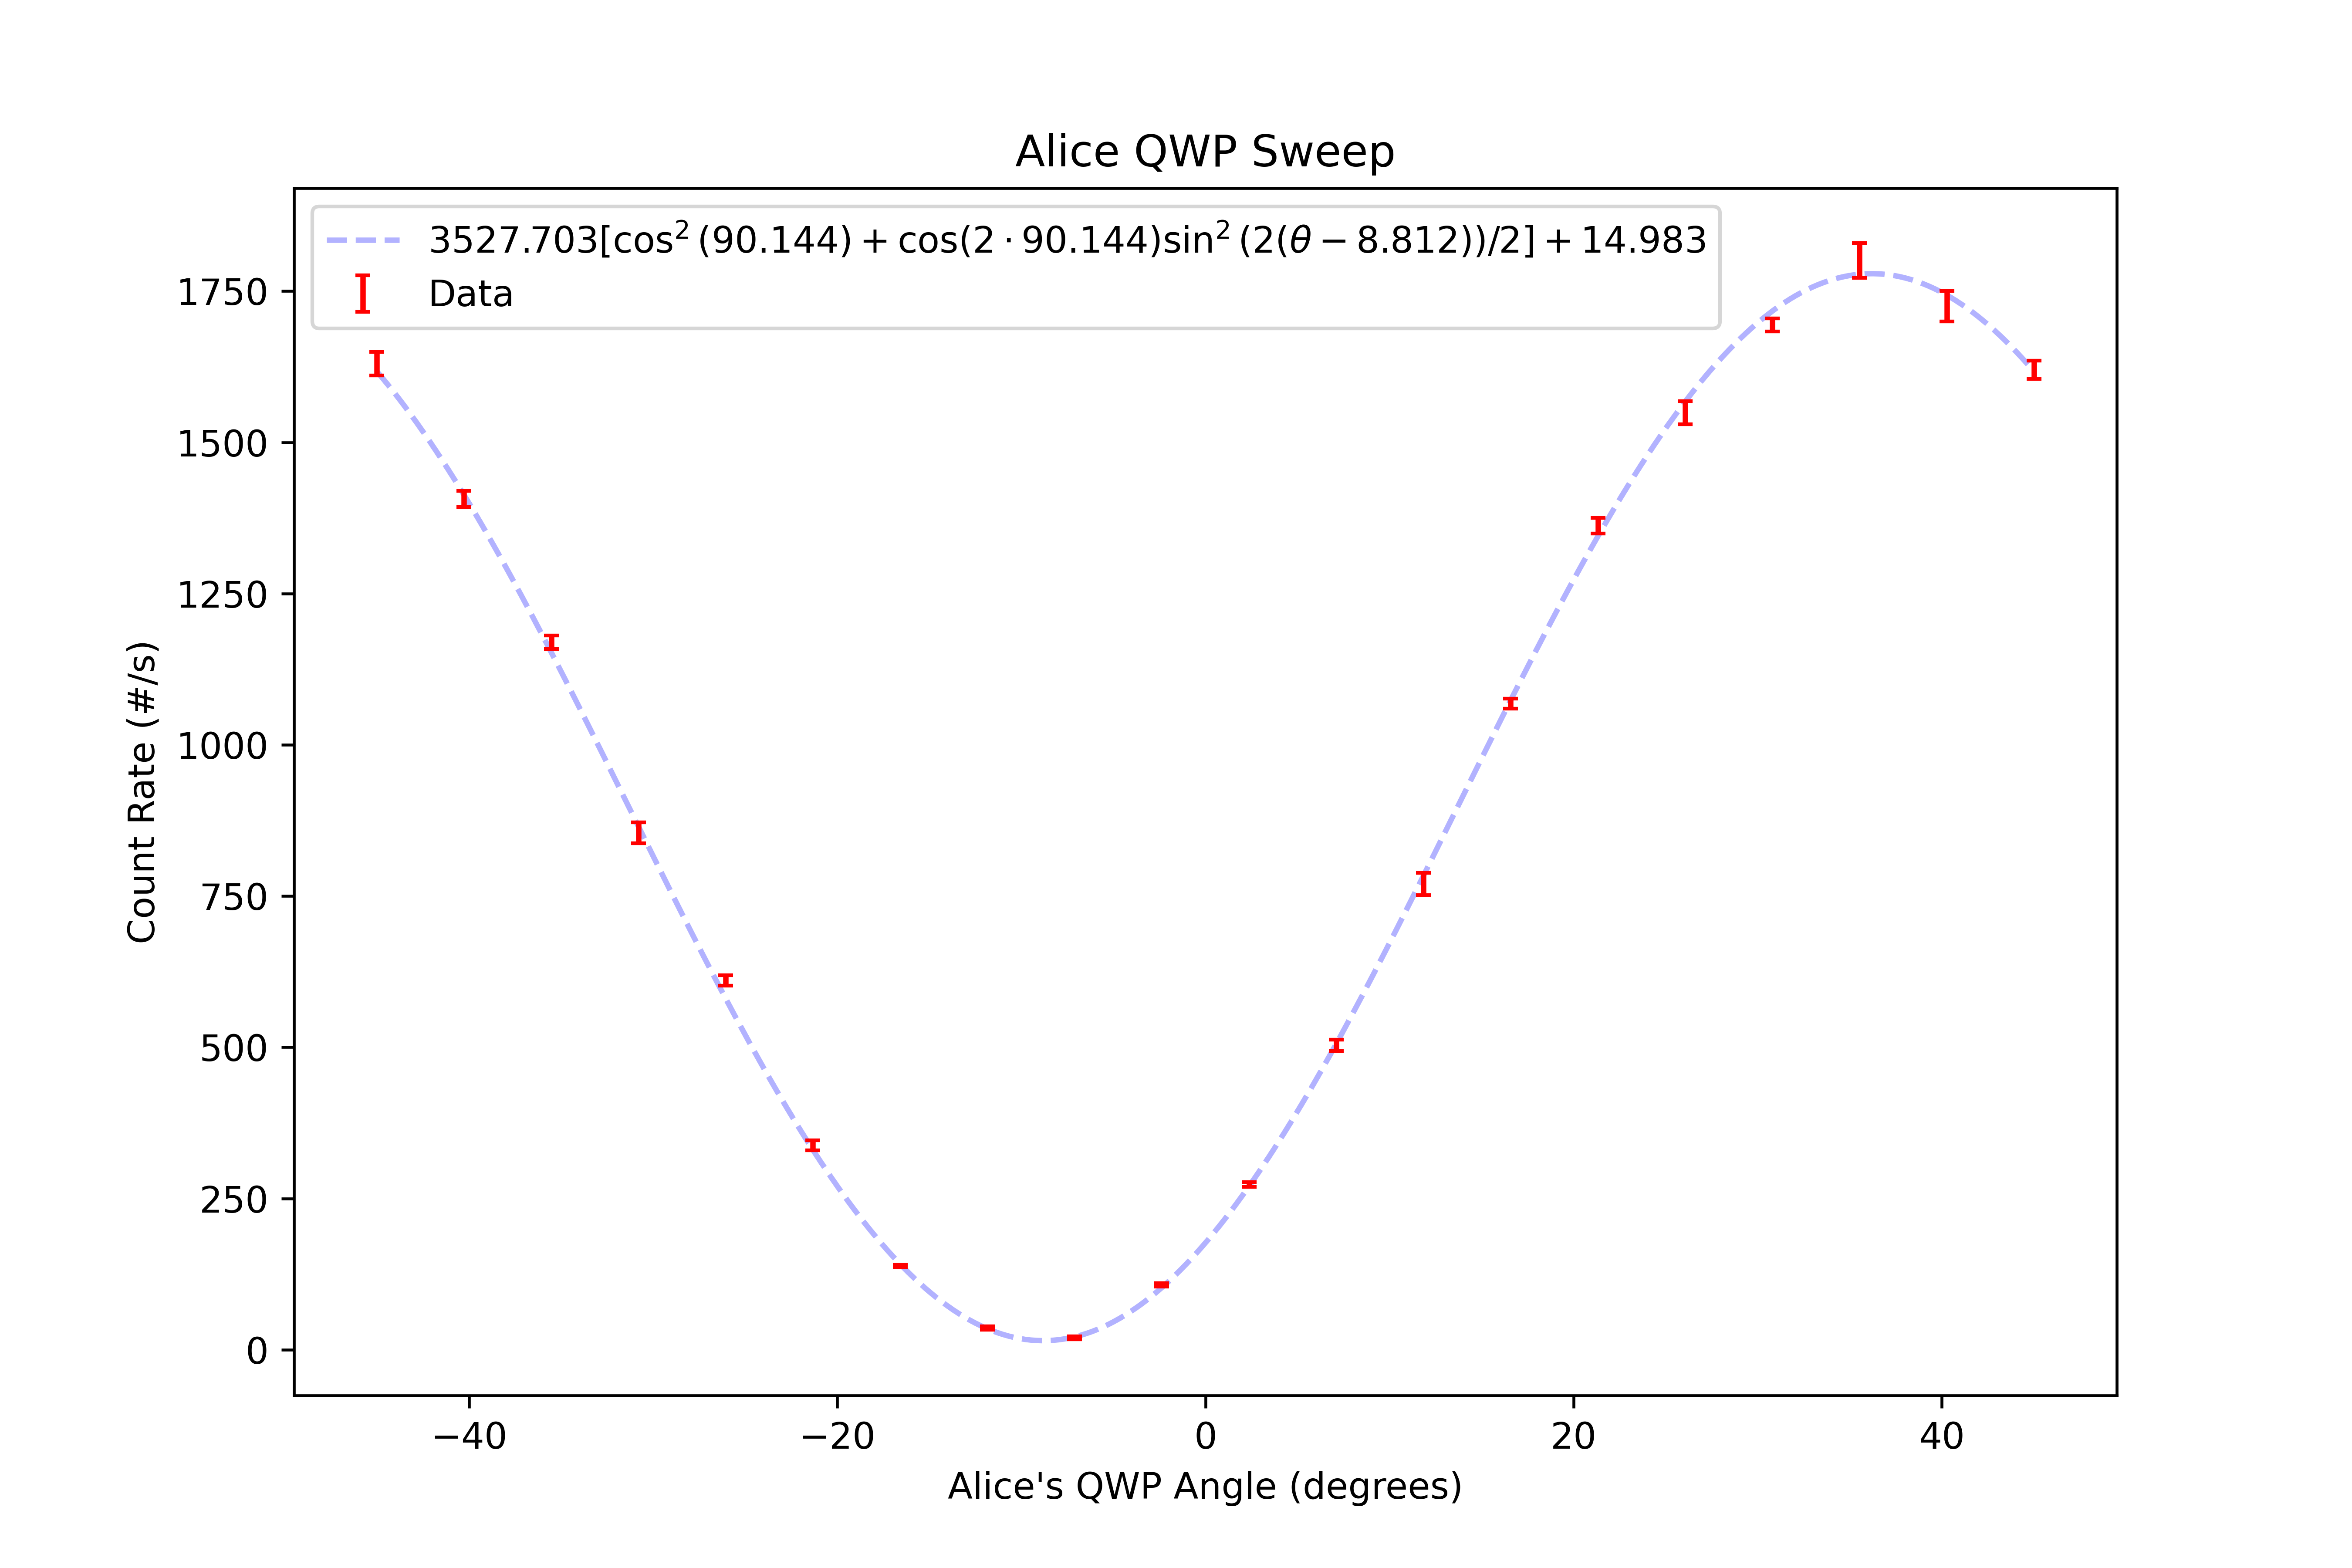
\includegraphics[width=0.9\textwidth]{AQWP/AQWP_fit.png}
		\caption{A coarse sweep of Alice's QWP when the UV HWP was set to its hardware's zero position. The minimum in this plot corresponds to the desired zero position for this motor. \textit{Note that Alice's HWP and the PBS have been removed for this trial.}}
		\label{fig:AQWP theory fit}
	\end{figure}
	This is the first step to the full calibration routine, playing with the UV HWP angle until we see that changing Alice's QWP angle significantly alters the count rates, then performing a sweep and fit of Alice's QWP to find where we achieve $\theta=0$. Note that we must remove Alice's HWP (which is on a magnetic mount) for these trials.
	
	Fitting to the theoretical function is more of a sanity check here. For the rest of the fits, we'll focus on the region around the minimum and stick to quadratic functions which give us an easy way to read off the extrema of any count rate data. Using this technique, \cref{fig:AQWP minimum fit} shows how we have determined the zero position for this motor is around $-8.704^\circ$ from the hardware home. \textit{Note that we will update this initial value (as well as all the others) during the checkpoints, so it likely will not match what is in the config.}
	
	\begin{figure}[p]
		\centering
		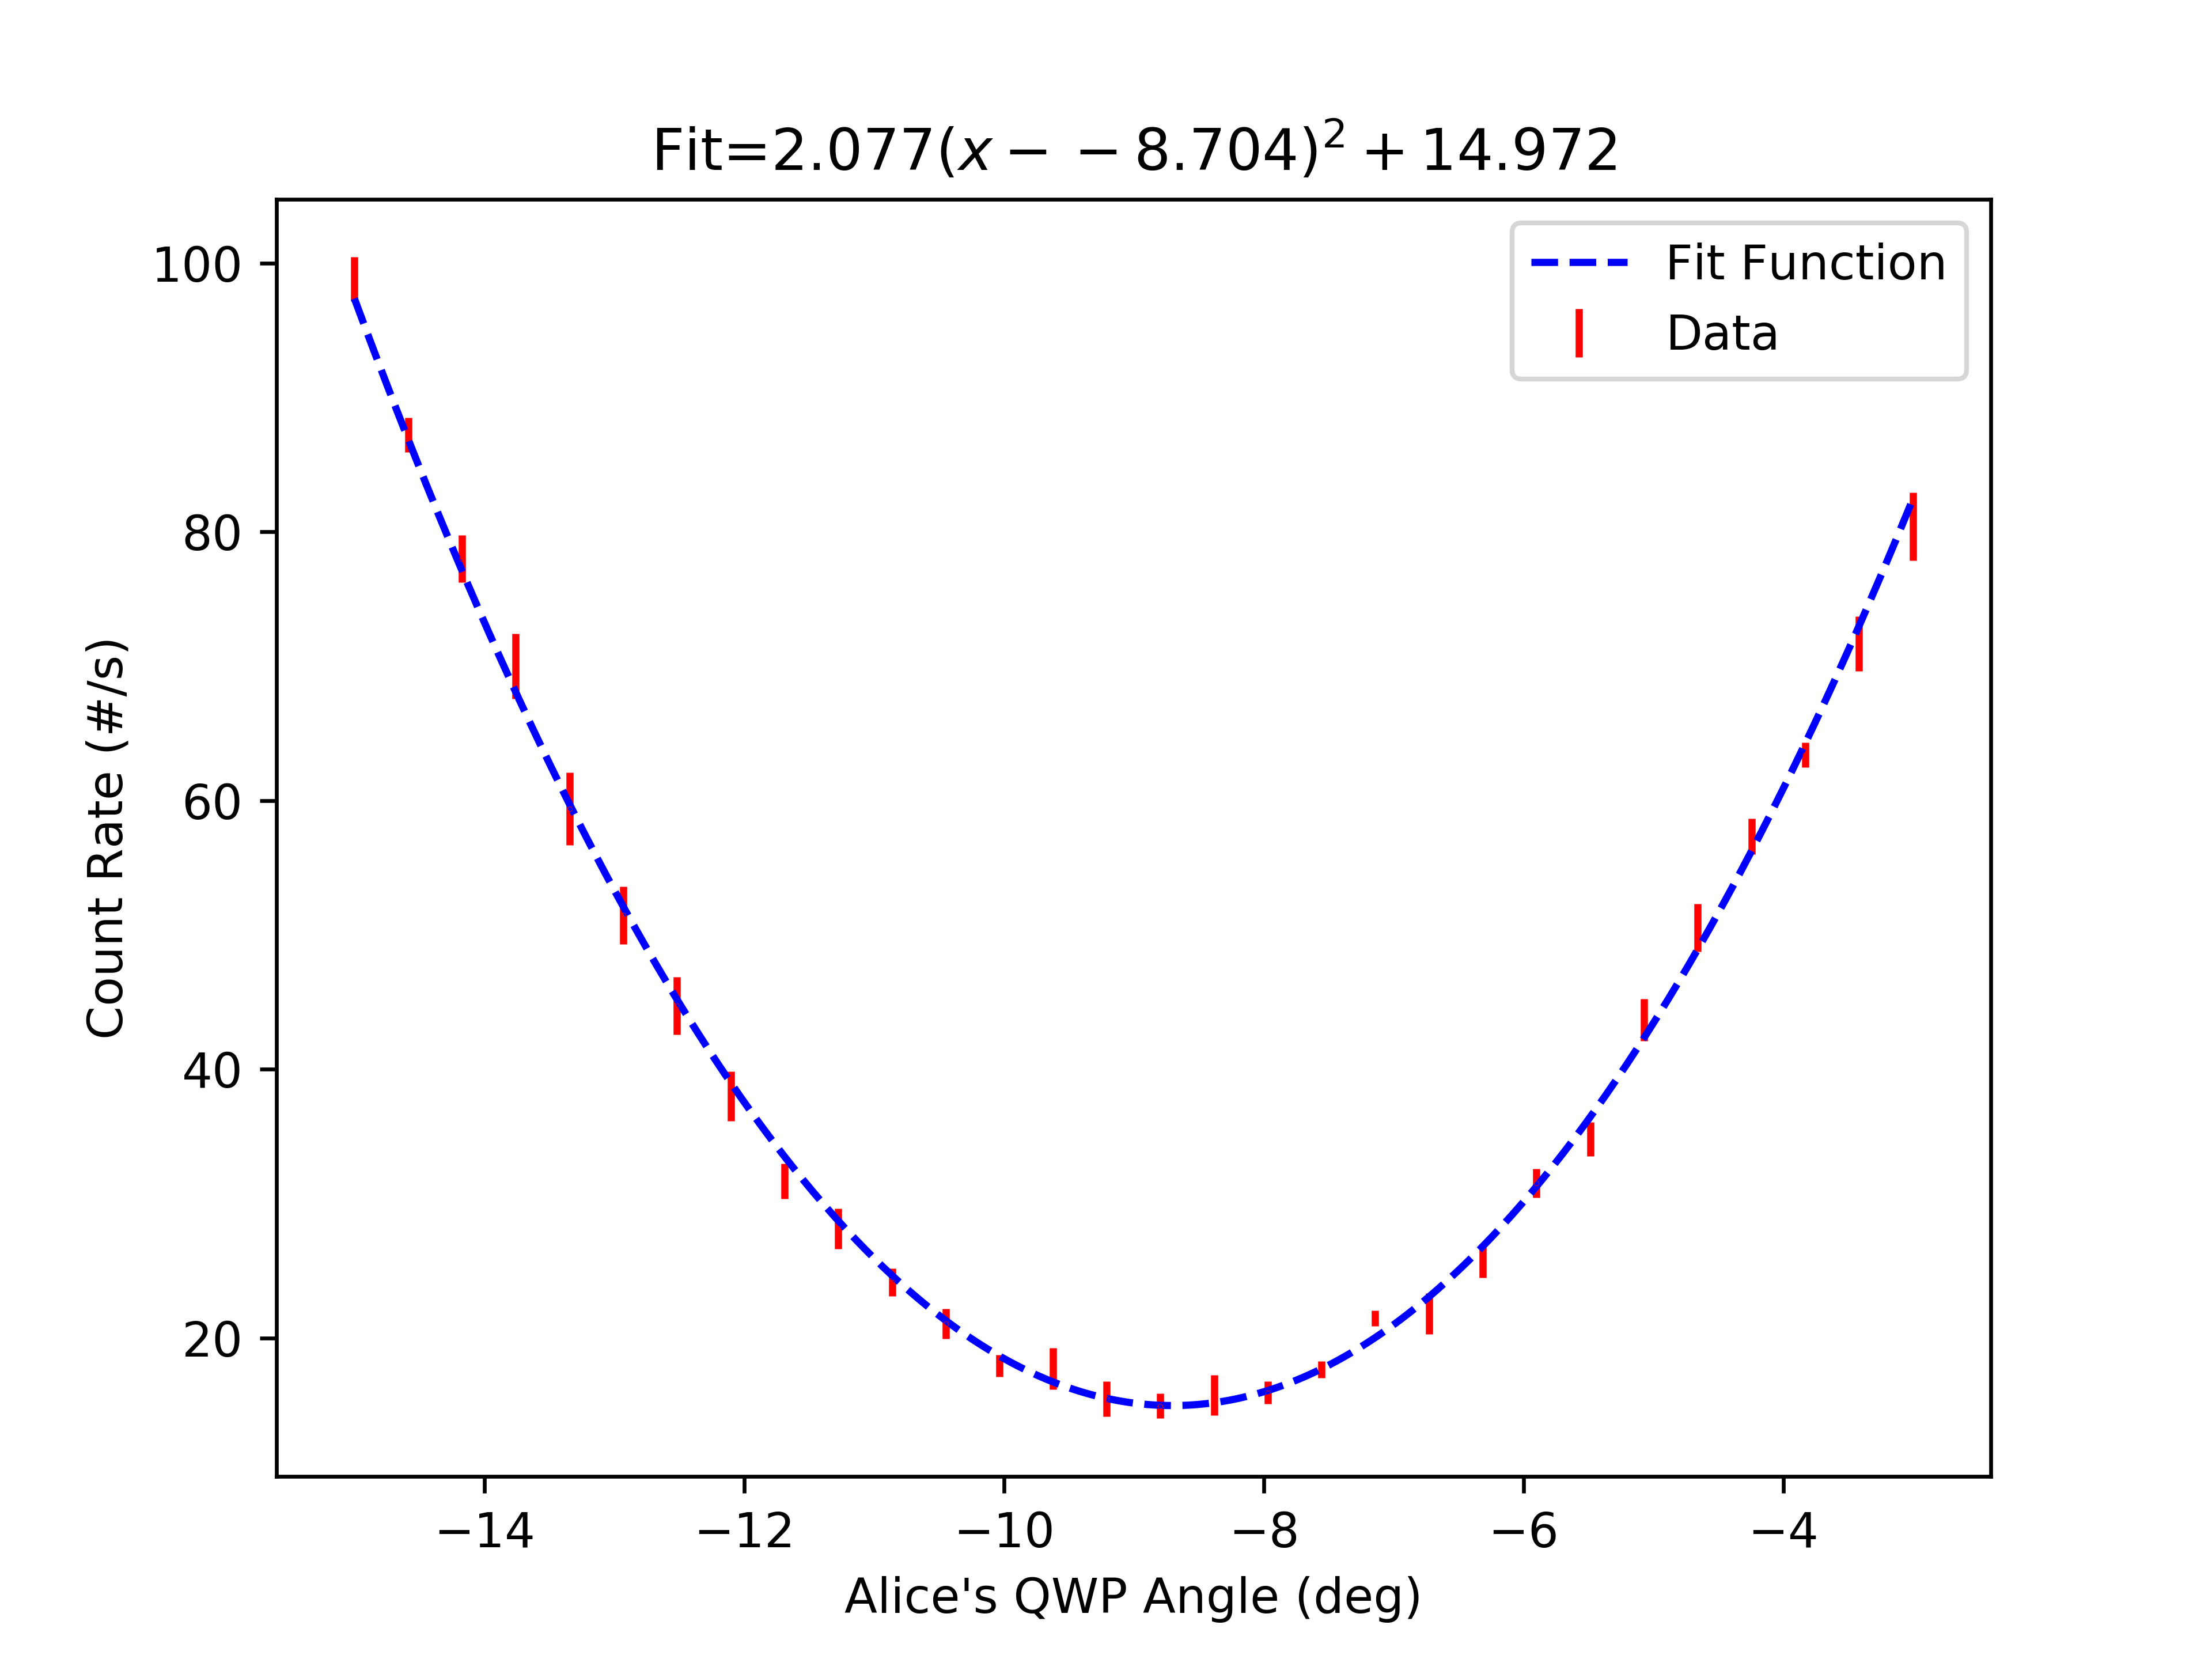
\includegraphics[width=0.9\textwidth]{AQWP/AQWP_sweep2.png}
		\caption{A fine sweep about the angle that minimizes the C4 count rates. \textit{Note that Alice's HWP and the PBS have been removed for this trial.}}
		\label{fig:AQWP minimum fit}
	\end{figure}
	
	\subsection{Calibrating the UV HWP}
	Once Alice's QWP can be set to a calibrated zero position, we can move it there and then mess with the UV HWP to find a minimum in the C4 detection rate. Since the QWP won't mess with linear polarizations, the minimum will be when the post-BBO state is simply $\VV$, meaning the UV HWP's fast axis makes an angle of $\theta=k\pi/2$ with the vertical. This is the method I used to find the UV HWP's offset as $-1.029^\circ$ from the hardware's home, the fit for which is shown in \cref{fig:UVHWP minimum fit}.
	\begin{figure}[p]
		\centering
		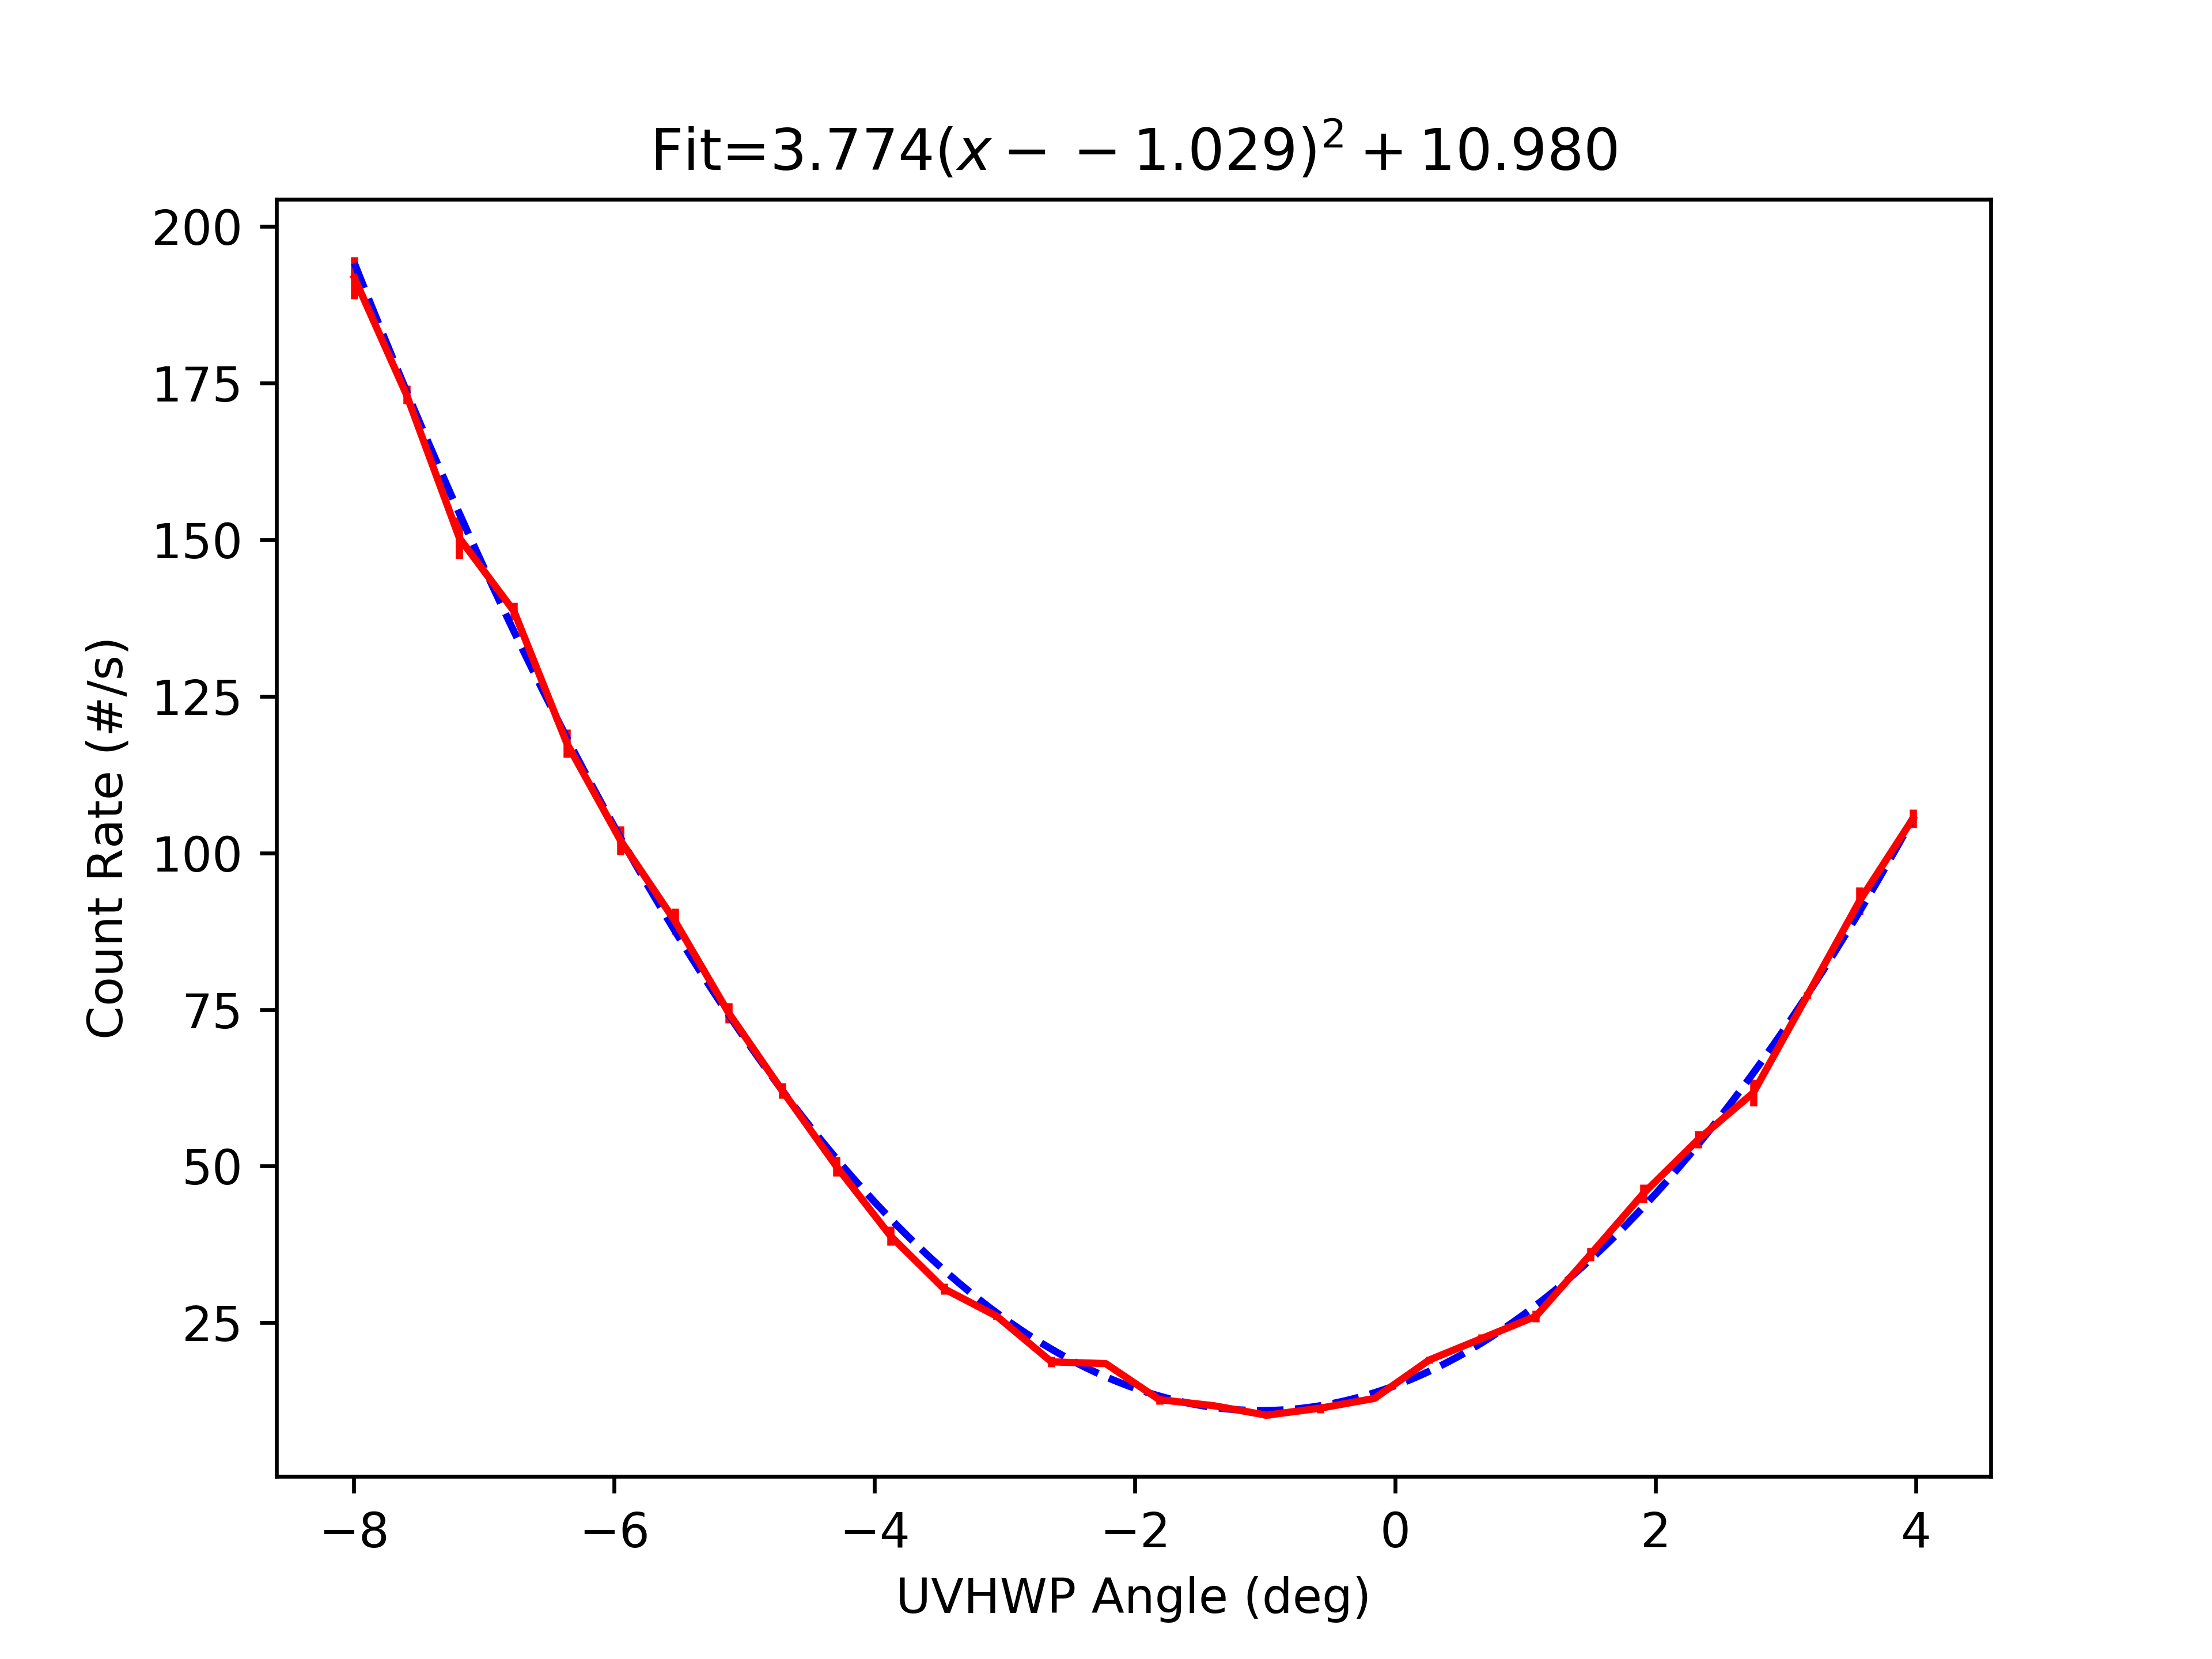
\includegraphics[width=0.9\textwidth]{UVHWP/UVHWP_sweep1.png}
		\caption{A fine sweep about the angle that minimizes the C4 count rates for the UV HWP while Alice's QWP is set to its calibrated zero position. \textit{Note that Alice's HWP and the PBS have been removed for this trial.}}
		\label{fig:UVHWP minimum fit}
	\end{figure}
	
	\subsection{Calibrating Alice's HWP}
	Once we have determined the zero position for Alice's QWP and are confident that we can produce the state $\VV$, we can sweep Alice's measurement HWP to find it's zero position. Since the state $\VV$ is separable, coincidence counts can be predicted directly from just Alice's photons. Specifically, if we are producing $\V$ and have correctly zeroed the QWP then we expect count rates of
	\begin{align}
		\avgt{C4}&=|\tb{H}\QWP_T(0)\HWP_T(\theta)\V|^2 \\
		&= \sin^22\theta
	\end{align}
	So we want to minimize these count rates in order to find the zero position for Alice's HWP ($\theta=0^\circ$). We can do this with the same coarse-then-fine sweeps we have been doing for the other motors. The fit for this data around the minimum is shown in \cref{fig:AHWP minimum fit}, and indicates that this motor should have an offset of $-9.470^\circ$ from the hardware home.
	
	\begin{figure}[p]
		\centering
		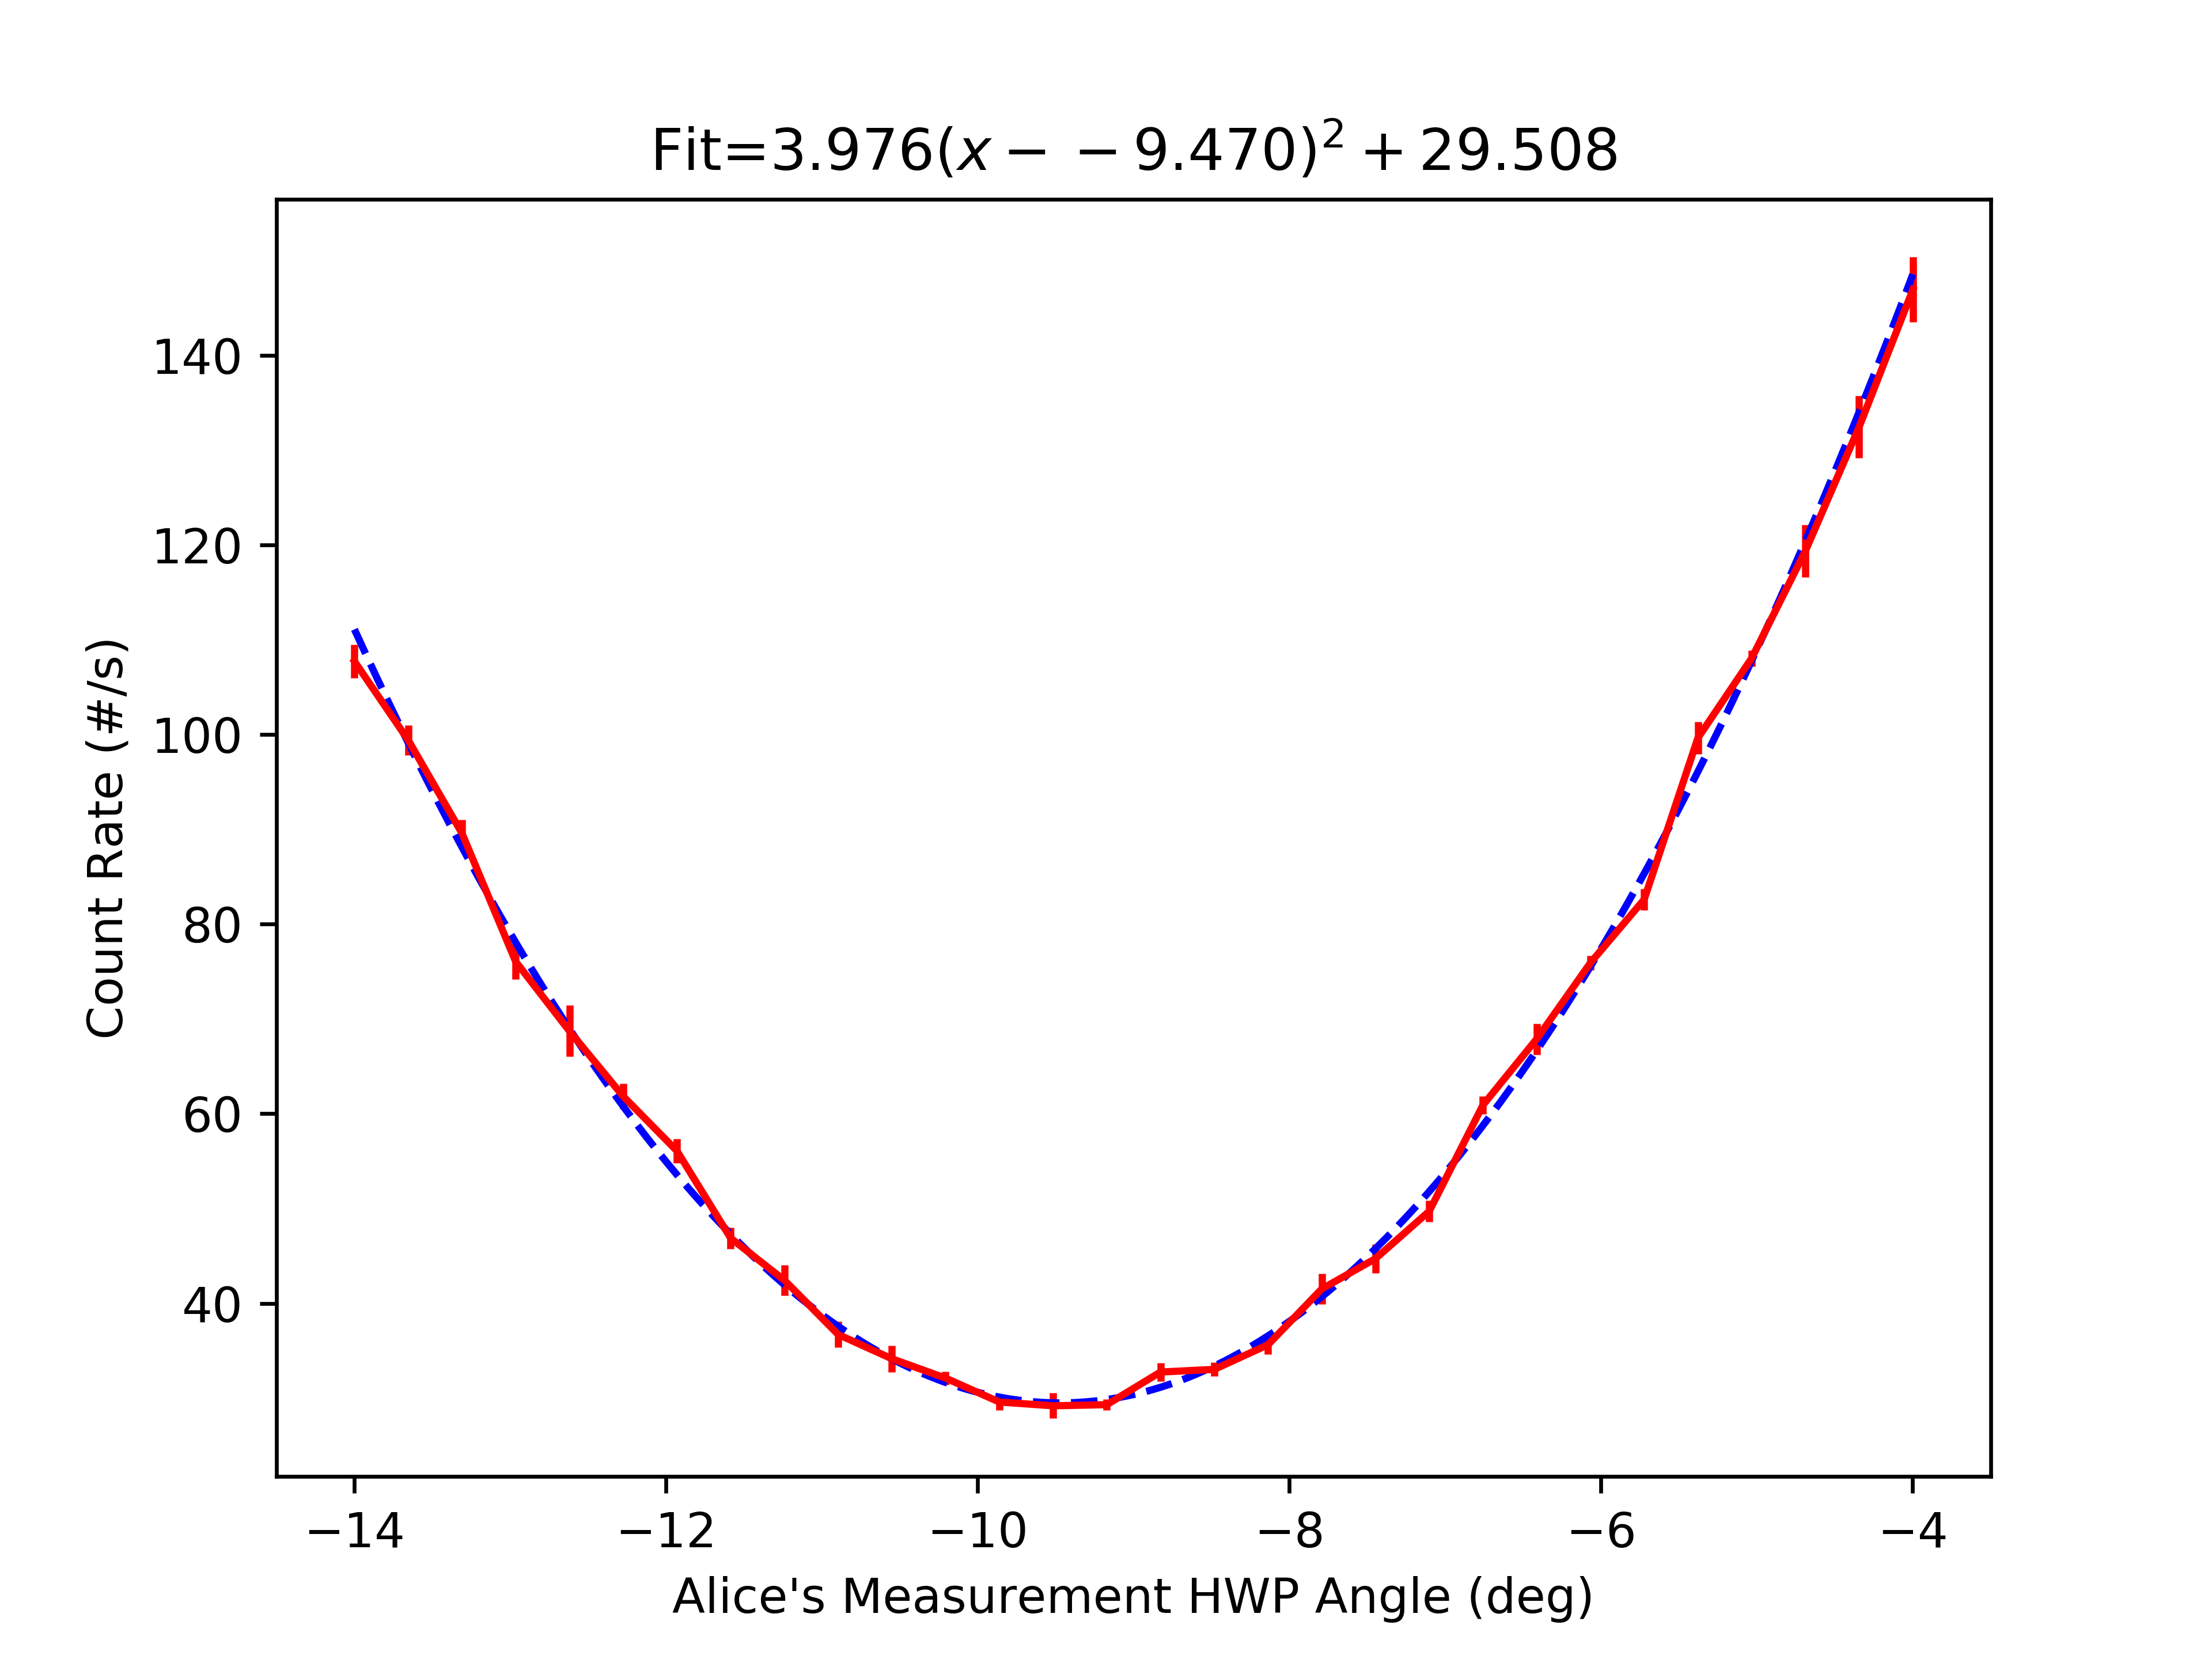
\includegraphics[width=0.9\textwidth]{AHWP/AHWP_sweep1.png}
		\caption{A fine sweep about the angle that minimizes the C4 count rates for the Alice's measurement HWP. \textit{Note that the PBS has been removed for this trial.}}
		\label{fig:AHWP minimum fit}
	\end{figure}
	
	\section{Checkpoint A}
	At this point, you should use the file \texttt{calibration/checka/check.py} to perform a check of all the calibration offsets that you have come up with so far. This file essentially just sets the UV HWP to produce $\VV$, then sets all of the wave plates on Alice's path to be at $0^\circ$, so that the C4 detection rate should be at a minimum. Then, one by one, it sweeps each component from $-4^\circ$ to $+4^\circ$ and plots the detection rate to confirm that there is a minimum at zero (finding the minimum using a quadratic fit).
	
	In our experience, the minimum will not necessarily be at zero right away. Likely, the measurement HWP will have a minimum at zero, but inserting it may have affected the minimum count rate positions of the UV HWP and measurement QWP.
	
	However, now that you know how much they got knocked off from zero, you can update the \texttt{offset} variables in the config files for each of the motors, and run the check again. This will likely be an iterative process. For our calibration, we had to run three separate sweeps before the results converged to minimum offsets of $<0.1^\circ$ for each motor. A summary of the changes made is shown in \cref{tab:checkpoint a}.
	\begin{table}[h]
		\centering
		\begin{tabular}{c||c|c|c|c}
		Motor & Initial ($^\circ$) & Final ($^\circ$) & $\Delta$ ($^\circ$) & New Minimum ($^\circ$) \\\hline
		UV HWP & $-1.029$ & $-1.381$ & $-0.352$ & $-0.006\pm0.022$ \\
		A HWP & $-9.470$ & $-9.351$ & $+0.119$ & $-0.022 \pm 0.018$\\
		A QWP & $-8.704$ & $-8.358$ & $-0.346$ & $-0.024\pm0.027$ \\
		\end{tabular}
		\caption{The changes that were made to the relevant motor offset positions thanks to the information provided by checkpoint A.}
		\label{tab:checkpoint a}
	\end{table}
	
	\subsection{Measuring Alice's Photon in the V Basis}
	
	We are about to calibrate Bob's wave plates in much the same way we did Alice's. However, it is a good idea to first make sure we can measure in bases like $\tk{V?}$, since we will still be producing $\VV$ and will want to be minimizing count rates for sweeps of Bob's quarter and half wave plates.
	
	For this purpose, there is a file \texttt{calibration/checka/measv.py} that performs a sweep of Alice's HWP around the angles in question and finds the one that maximizes detections (which should be 45$^\circ$ from the calibrated zero position).
	
	\section{Bob's Wave Plates}
	
	Now we'll turn our attention back to Bob's photon and his wave plates. Firstly, we will need to put Bob's PBS back in so that we can make meaningful measurements of his photon. The general strategy here will be the same as it was for Alice. We'll put Alice's wave plates into a calibrated position to measure her photon in the V basis while producing $\VV$, and then by finding where the fast axis of each of Bob's wave plates is either horizontal or vertical, we will be minimizing C4 coincidence count rates.
	
	\subsection{Procedure}
	The process for Bob's wave plates is essentially the same as it was for Alice's HWP. Now that we have tuned the UVHWP during checkpoint A, we will not be messing with the offset for that wave plate any further, which means for each of Bob's wave plates we essentially just do the a basic coarse then fine sweep to determine the position that minimizes C4 coincidence counts. The one tricky part is we do have to complete this process one-by-one for each wave plate, and since a number of the wave plates are screwed down, we should try to be thoughtful about the order. Here is the order that we did things in:
	\begin{enumerate}
		\item Remove all wave plates on Bob's path except for the measurement QWP.
		\item Run the sweep to find the correct offset for this Bob's measurement QWP.\footnote{This wave plate is of particular note because it is mounted with its fast axis ~90$^\circ$ from the zero position. This can be confusing, since there will also be a minimum of C4 counts around 0$^\circ$, but the one at ~90$^\circ$ is where the fast axis is mounted horizontally.} A plot of this data is shown in \cref{fig:BQWP minimum fit}, and indicates that the desired zero position of this motor is $88.807^\circ$.
		\item Run red light through the detector, and align the QWP by making sure it is retro-reflecting. Install the measurement HWP on the magnetic mount, align it, and then remove it gently. Install Bob's creation HWP (remembering to leave room for the creation QWP) and align it.
		\item Run the sweep to determine the correct offset for Bob's creation HWP that leaves the fast axis vertical. The sweep I performed for this component is shown in \cref{fig:BCHWP minimum fit} and indicates a zero position of $-0.044^\circ$.
		\item Put the measurement HWP on the magnetic mount back into the photons path, then run the sweep for this wave plate (this time determining where the fast axis is on the horizontal). The sweep performed is shown in \cref{fig:BHWP minimum fit}, and indicates a zero position of $-15.624^\circ$.
		\item Finally, we would want to install the creation QWP (aligning it as necessary) and run the sweep for this component to find where its fast axis is vertical. On July 20th, 2023, we ran some tests that showed the creation QWP was loose inside of its aluminum housing. For the time being, we are leaving it uninstalled.
	\end{enumerate}
	
	\begin{figure}[p]
		\centering
		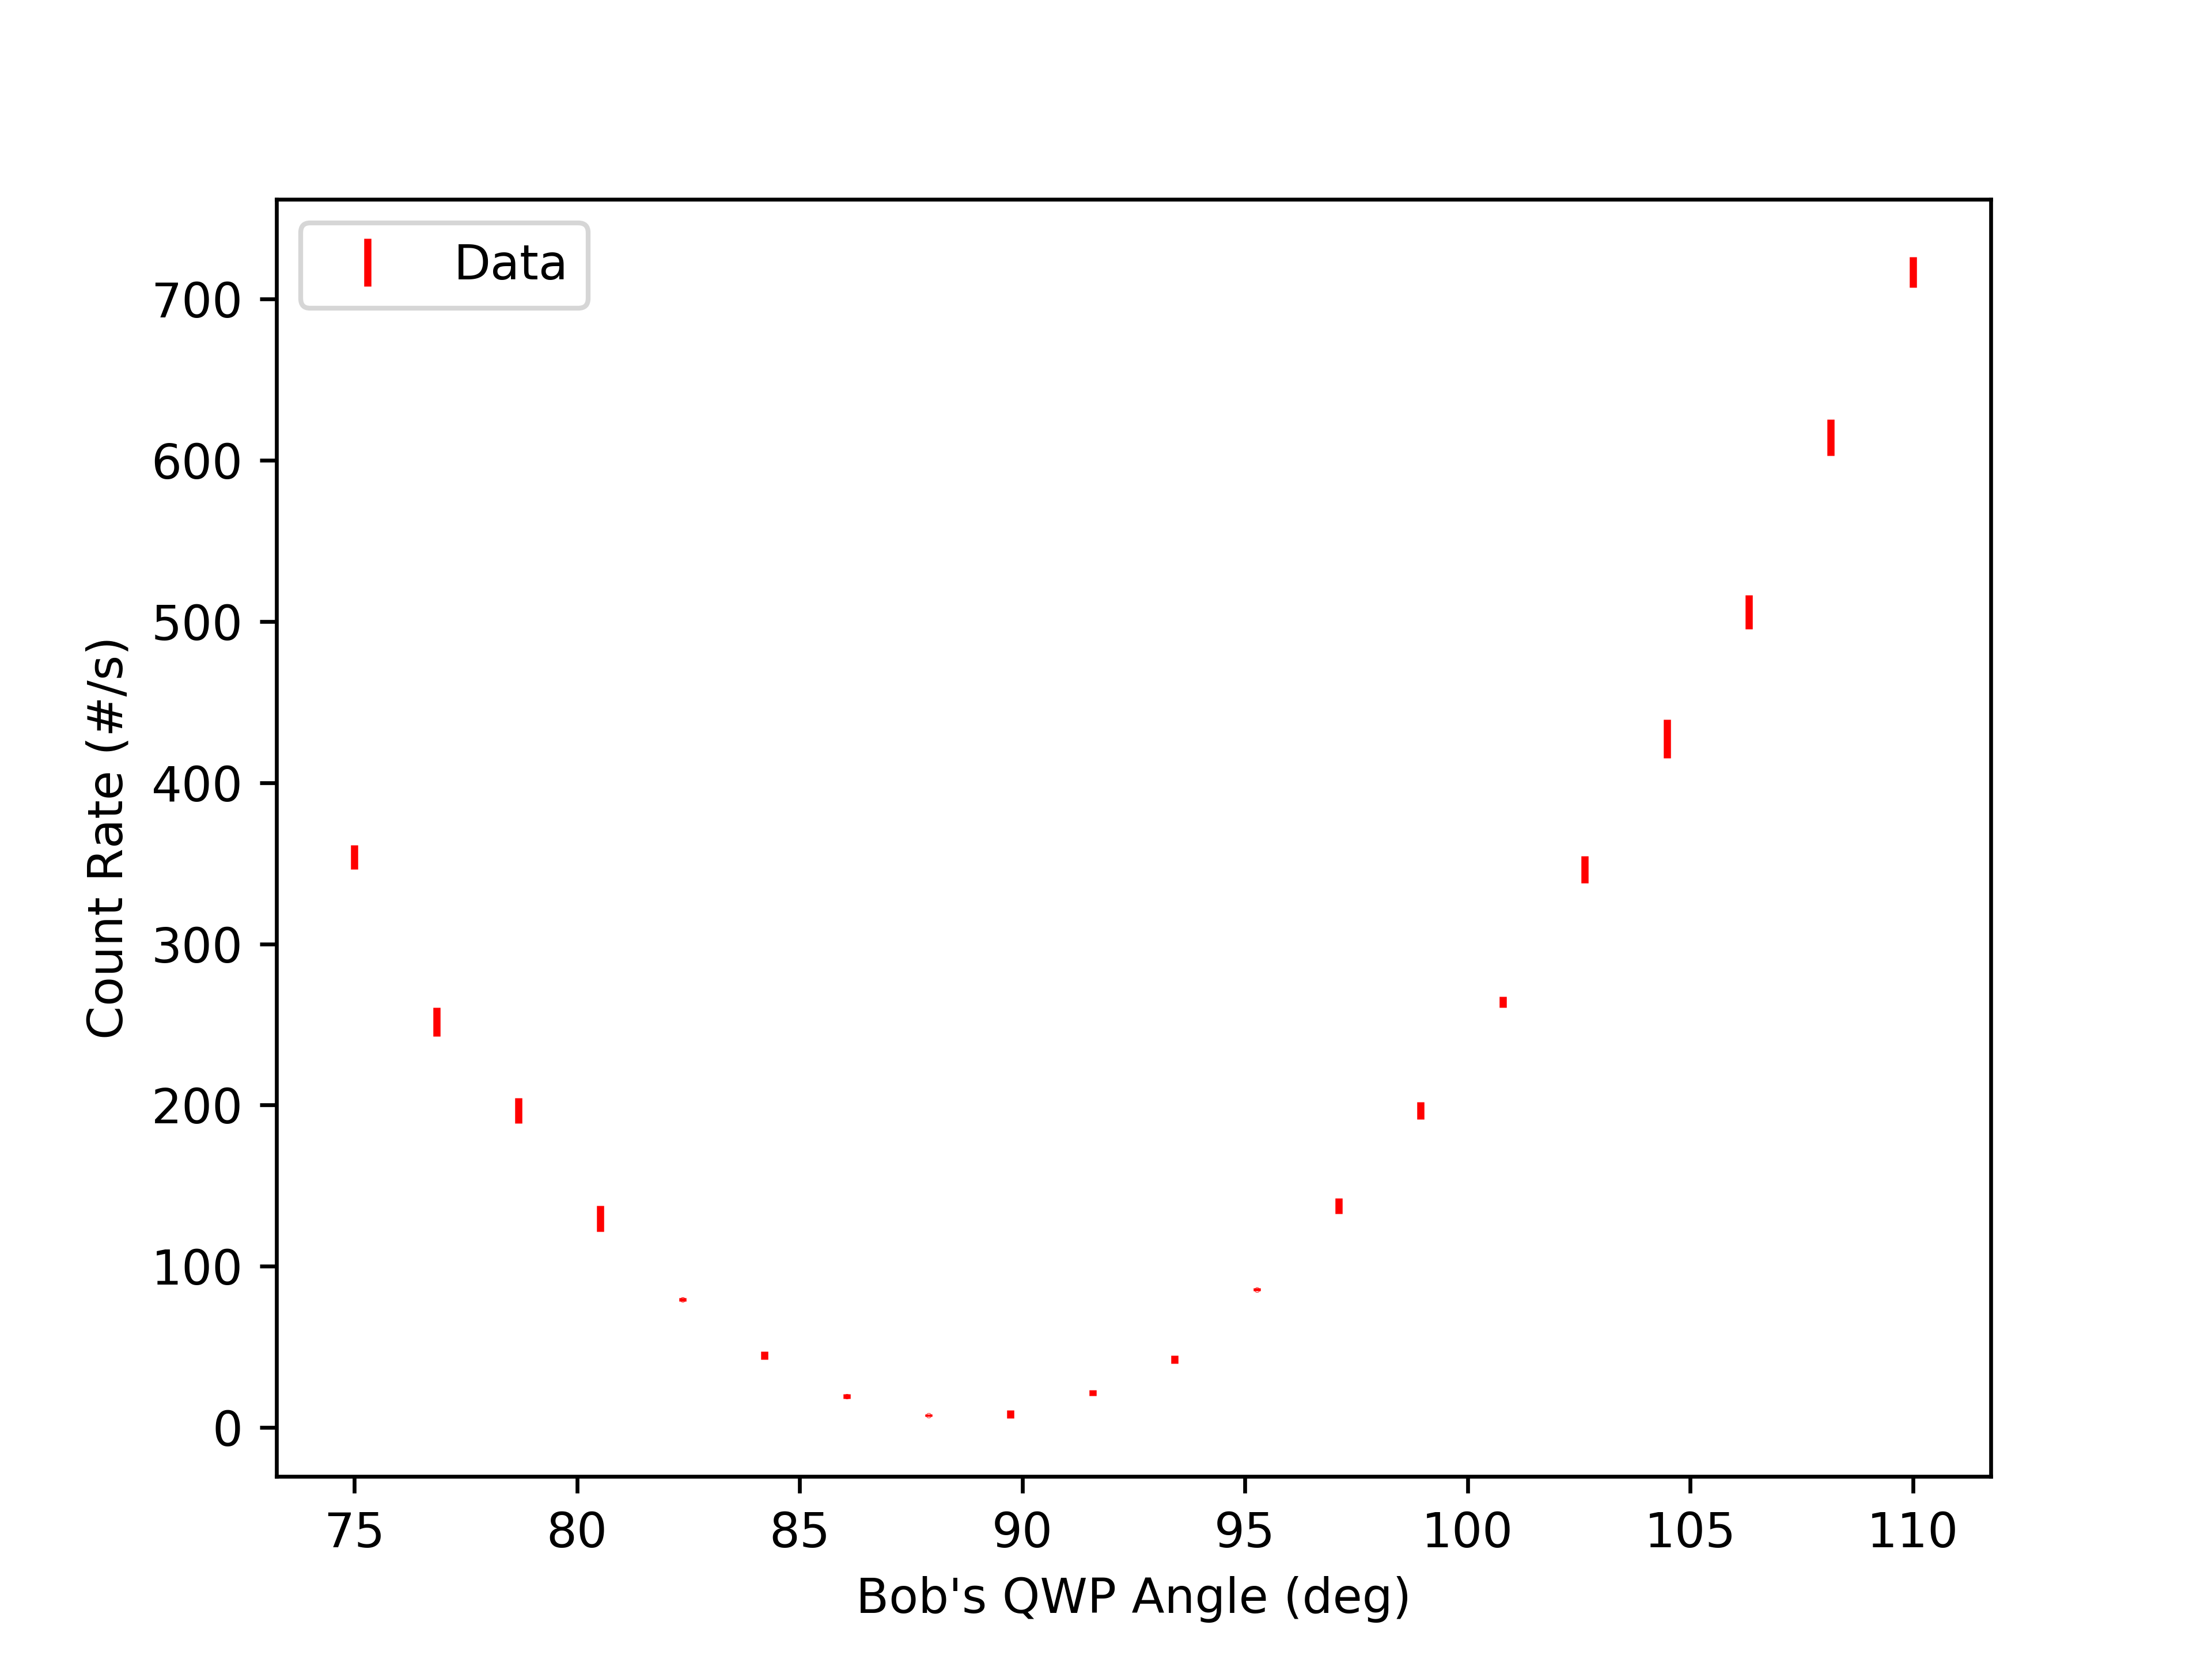
\includegraphics[width=0.9\textwidth]{BQWP/BQWP_sweep0.png}
		\caption{A fine sweep about the angle that minimizes C4 count rates for the Bob's measurement QWP. Alice's wave plates have been configured to allow detection of the $\V$ state for this trial.}
		\label{fig:BQWP minimum fit}
	\end{figure}
	\begin{figure}[p]
		\centering
		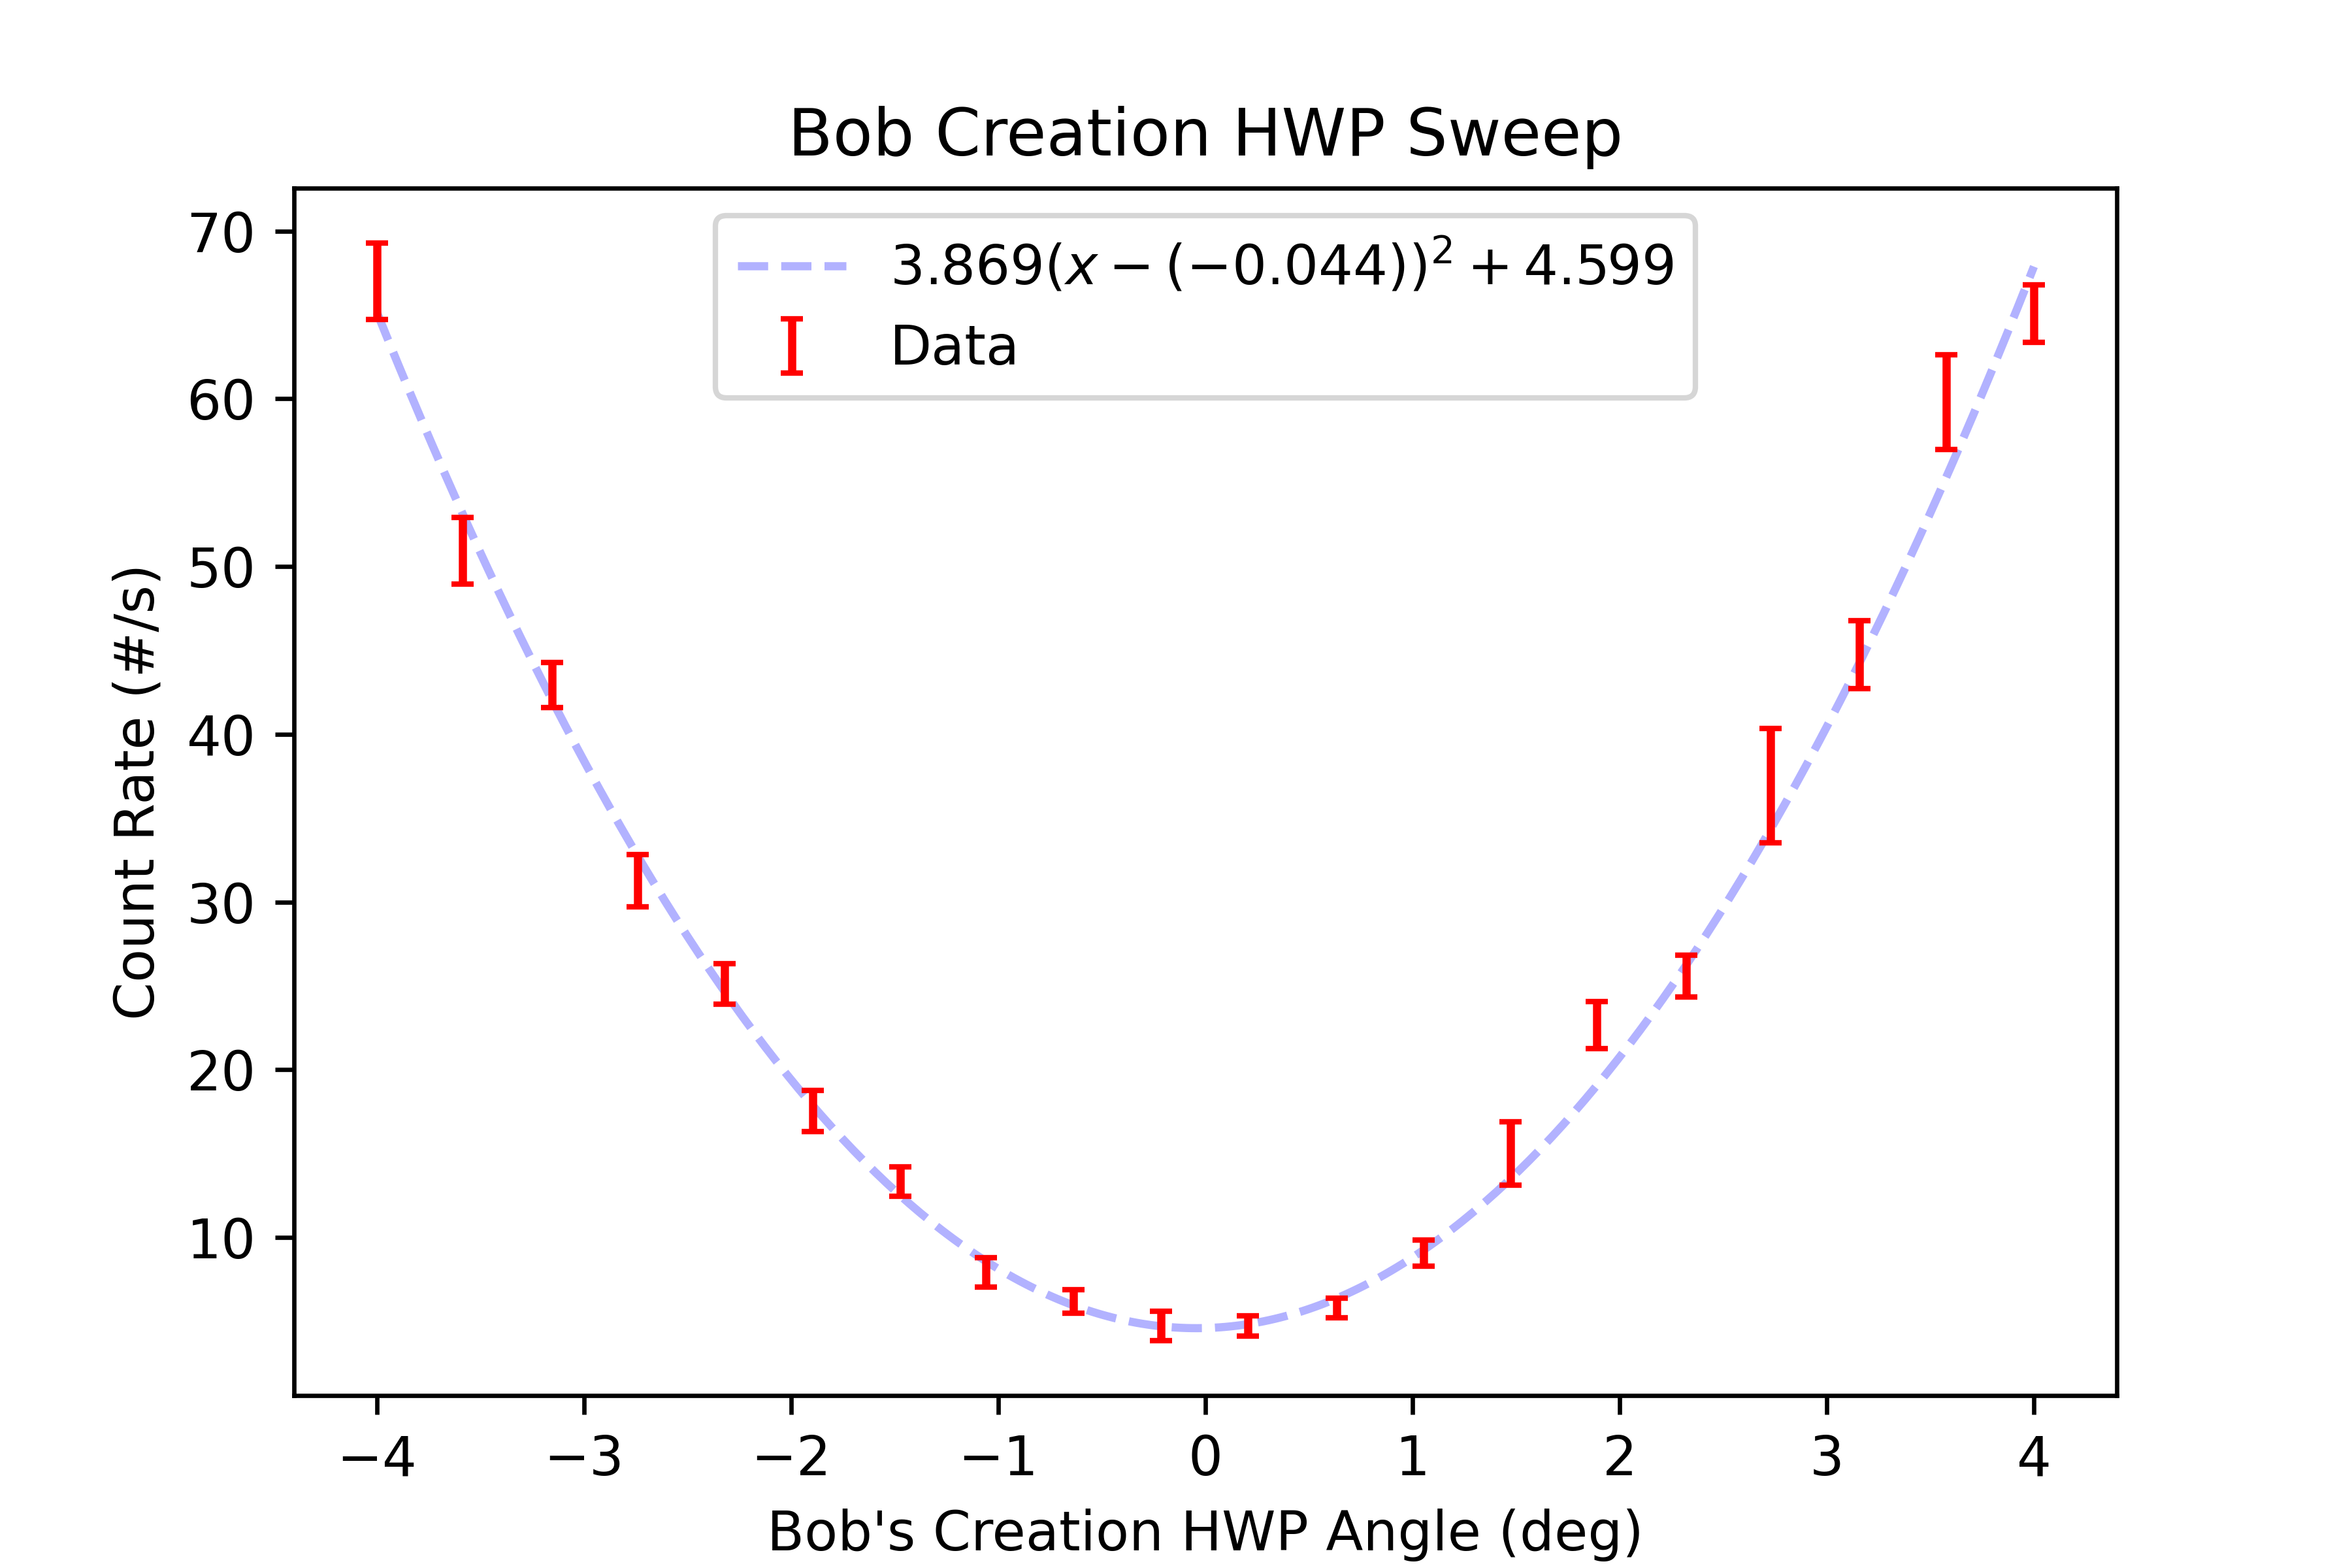
\includegraphics[width=0.9\textwidth]{BCHWP/BCHWP_sweep0.png}
		\caption{A fine sweep about the angle that minimizes C4 count rates for the Bob's creation HWP. Alice's wave plates have been configured to allow detection of the $\V$ state for this trial.}
		\label{fig:BCHWP minimum fit}
	\end{figure}
	\begin{figure}[p]
		\centering
		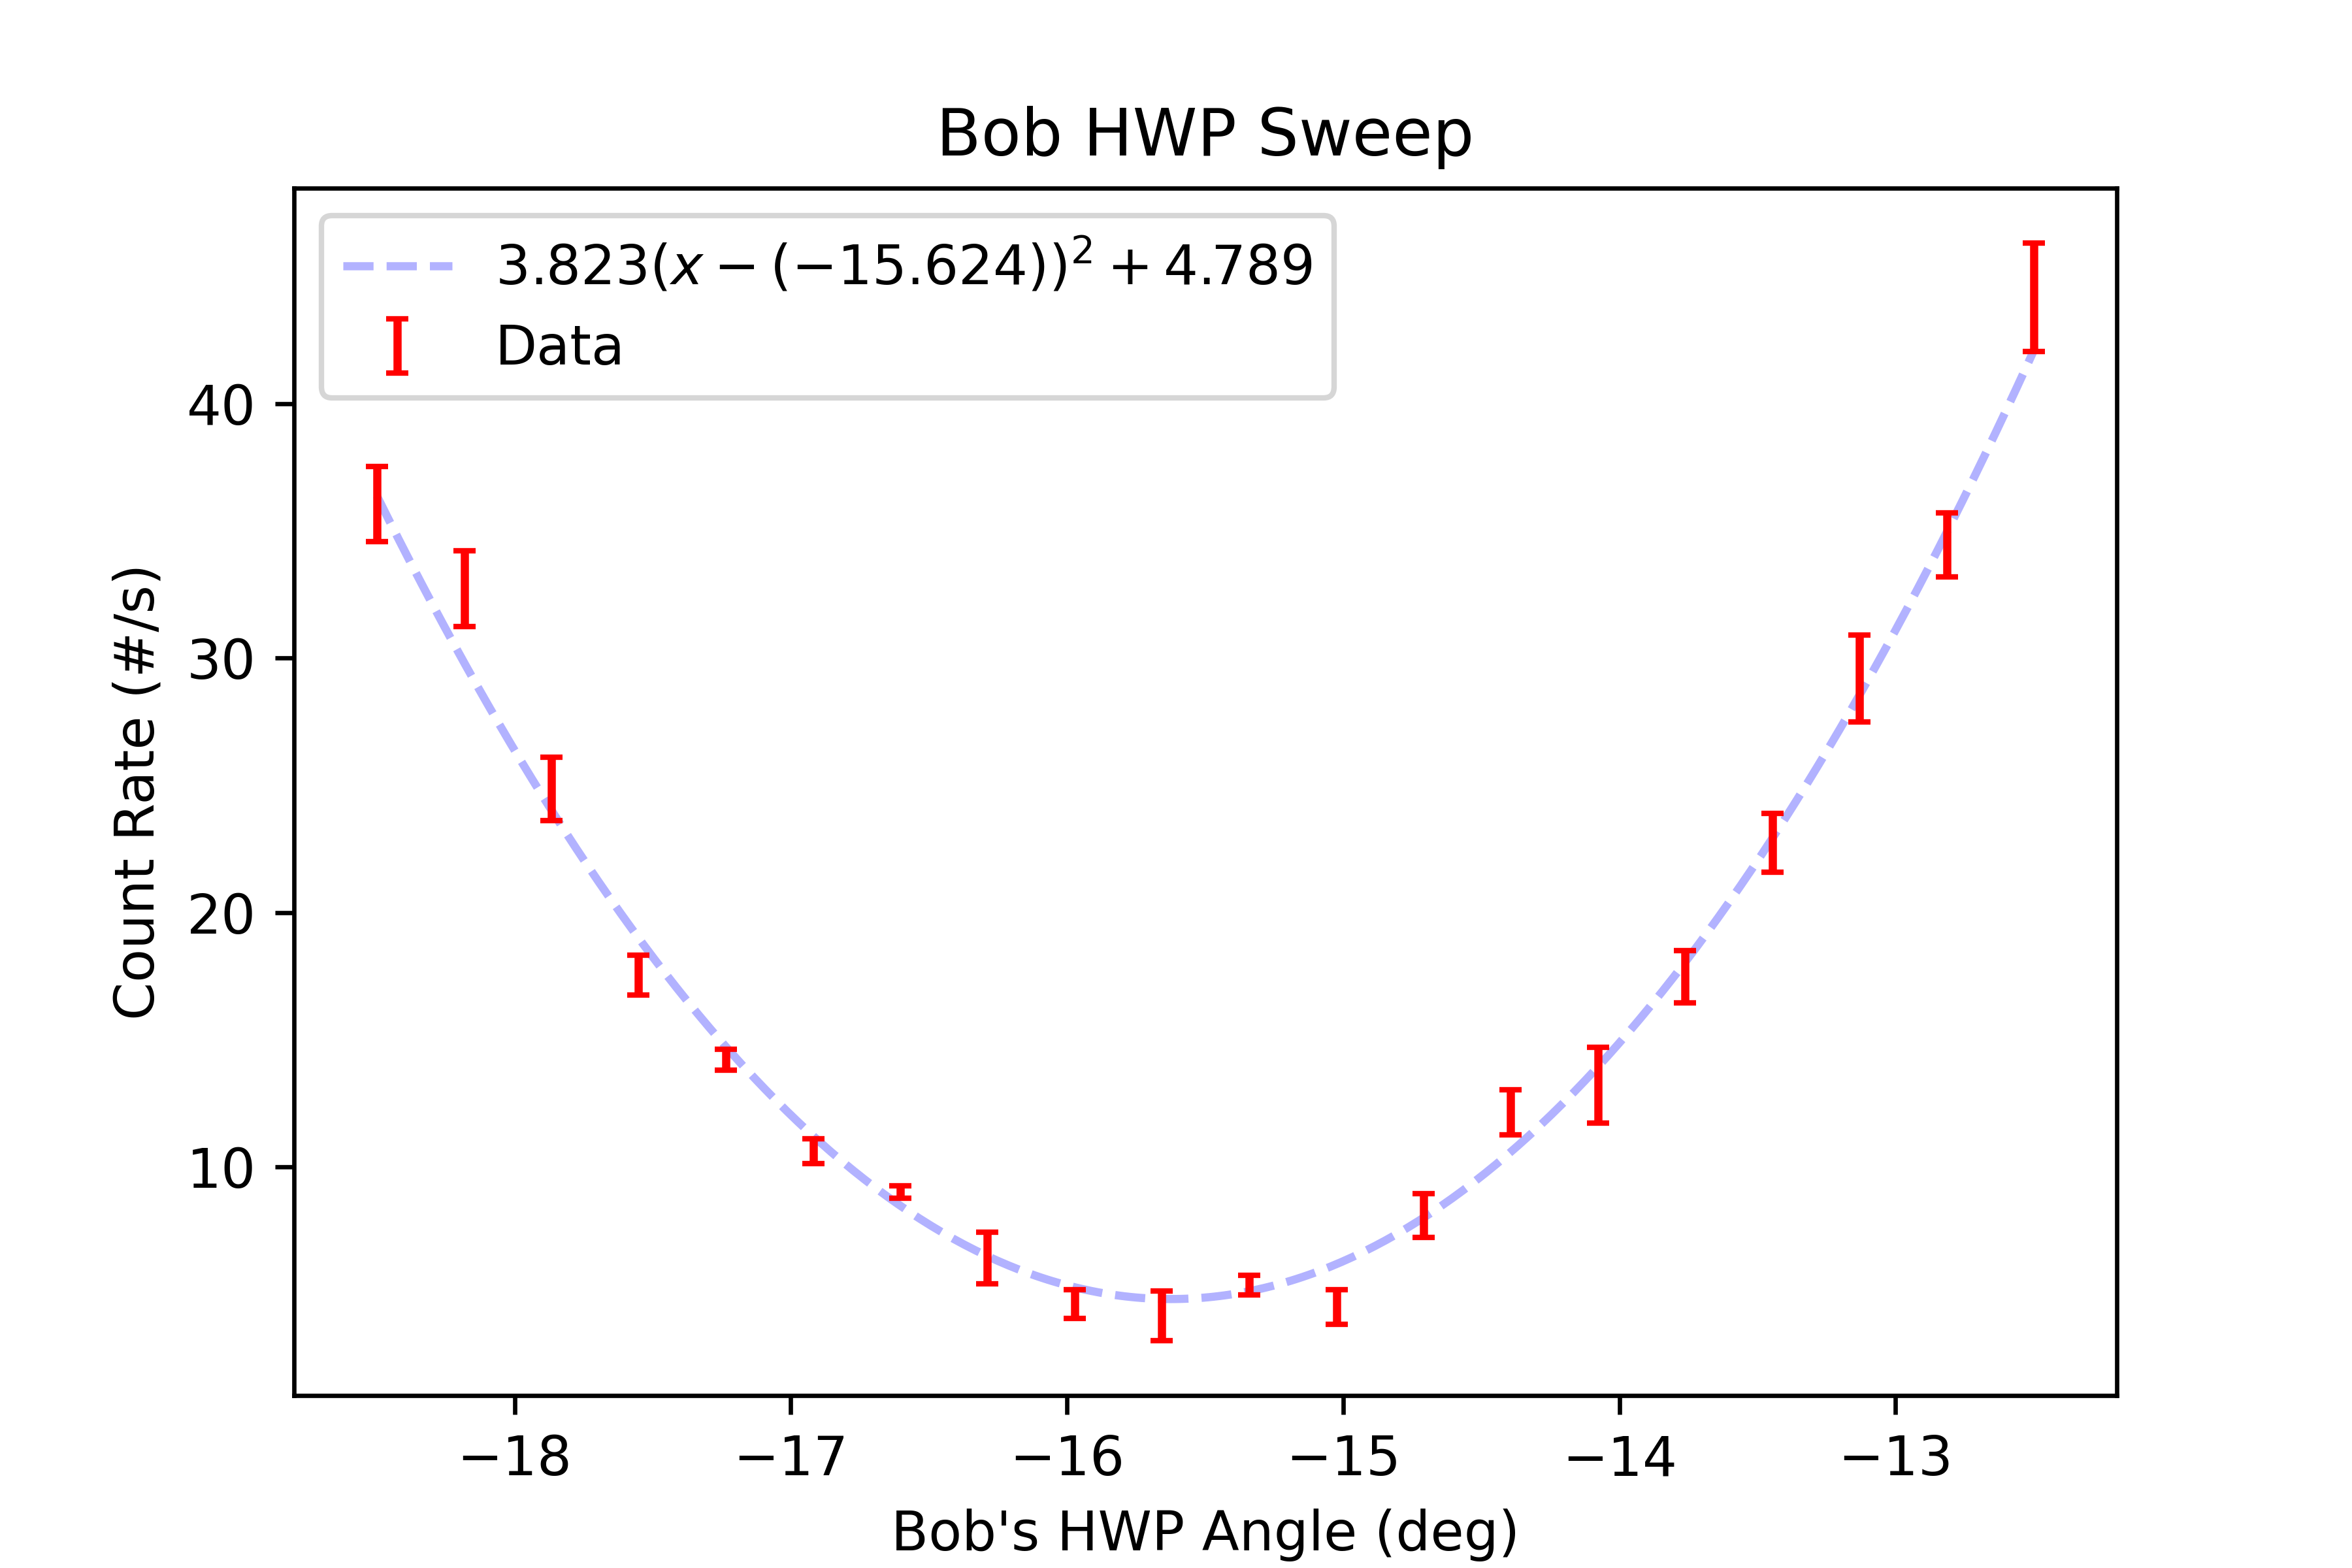
\includegraphics[width=0.9\textwidth]{BHWP/BHWP_sweep2.png}
		\caption{A fine sweep about the angle that minimizes C4 count rates for the Bob's measurement HWP. Alice's wave plates have been configured to allow detection of the $\V$ state for this trial.}
		\label{fig:BHWP minimum fit}
	\end{figure}
	
	\section{Checkpoint B}
	Checkpoint B is designed to perform the same task as checkpoint A, but for Bob's wave plates. We set up the state $\VV$, set Alice's HWP to $45^\circ$ so that we measure her photon in the $\V$ basis, and align all of Bob's wave plates to $0^\circ$ to minimize C4 detection counts.
	
	This checkpoint seems to be a fair bit more stable than checkpoint A, and much more in agreement with all the measurements leading up to it. By that I mean to say that we didn't actually adjust any of the zero positions as they were determined by the sweeps. The checkpoint indicated that all of the minima were within our semi-arbitrary margin of error of $0.1^\circ$.
	\begin{table}[h]
		\centering
		\begin{tabular}{c||c}
			Component & Minimum (${}^\circ$) \\\hline
			BQWP & $0.083 \pm 0.020$ \\
			BHWP & $-0.033 \pm 0.014$ \\
			BCHWP & $0.003 \pm 0.015$
		\end{tabular}
		\caption{The minimum count positions found by checkpoint B. No updates were made since all minima were less than $0.1^\circ$.}
	\end{table}
	
	\section{Phi Plus}
	The last component to calibrate is the pre-compensation crystal (PCC). The affect of this crystal is to reduce the phase-smearing affect of the BBO effectively by smearing the phase in the opposite way before the light hits the BBO. In order to consider the phase smearing at all though, we will need to create a superposition state that is some combination of $\HH$ and $\VV$ (up until now, we've only been considering the separable state $\VV$. A particularly nice state to work with is
	\begin{equation}
		\ket{\Phi^+}=\frac{\HH + \VV}{\sqrt{2}}
	\end{equation}
	We will now calibrate this state.
	
	\subsection{Determining the Phase Difference}
	By leaving Bob's creation wave plates at their calibrated zeros, linear polarizations $\HH$ and $\VV$ coming from the BBO remain linear. The general form of a state will be something like
	\begin{equation}
		\ket{\Psi} = \cos\theta\HH + i e^{i\phi_0}\sin\theta\VV \label{eq:general hh vv state}
	\end{equation}
	Where $\tan^2\theta$ is the ratio of $\VV$ to $\HH$ and $\phi_0$ is the phase imparted on the state by the quartz plate. Note the latent $i$ on the $\VV$ term - this comes from the fact that Bob's horizontally polarized photon will pick up a factor of $-i$ while traveling along the slow axis of the creation half and quarter wave plates, which is equivalent to the vertically polarized photon picking up a factor of $i$. However, we will just bundle this into the phase term $\phi=\phi_0+\pi/2$ so that the general state looks like
	\begin{equation}
		\ket{\Psi} = \cos\theta\HH + e^{i\phi}\sin\theta\VV
	\end{equation}
	From this, we can calculate the expectation values
	\begin{align}
		\eDR=\eAL &= \frac{1+\sin\phi\sin2\theta}{4} \\
		\eDL=\eAR &= \frac{1-\sin\phi\sin2\theta}{4} \\
		\eRR=\eLL &= \frac{1-\cos\phi\sin2\theta}{4} \\
		\eRL=\eLR &= \frac{1+\cos\phi\sin2\theta}{4}
	\end{align}
	Which tells us that we can calculate the phase $\phi$ as
	\begin{equation}
		\phi = \arctantwo\left(\frac{\eDR-\eDL-\eAR+\eAL}{-\eRR+\eRL+\eLR-\eLL}\right)\in(-\pi,\pi]
	\end{equation}
	
	I am mentioning the phase first because it is important to get the phase difference between these two terms correct before attempting to narrow in on the ratio of $\HH$ to $\VV$s. This is because the quartz plate has different indexes of refraction for horizontal and polarization, and so changing the angle of the quartz plate will change the amount of light of each polarization that gets reflected, thus changing the ratio of $\HH$ to $\VV$. Thus, the first step to calibrating $\ket{\Phi^+}$ is to set the UV HWP to $45^\circ$ so that we see some decent amount of $\HH$ and $\VV$, then performing a sweep of the quartz plate to measure the phase as a function of quartz plate angle.
	
	\subsection{HH:VV Ratio}
	Once we have determined where the phase shift between the two terms is equal to zero, we can fine-tune the ratio of $\HH$ to $\VV$ to get exactly one-half. Since we should not assume perfect calibration or performance of Bob's creation wave plates, we should use the following formula to get the ratio in terms of $\theta$
	\begin{equation}
		\theta = \arctan\sqrt{\frac{\eVH+\eVV}{\eHH+\eHV}} \in \left[0,\frac{\pi}{2}\right]
	\end{equation}
	Then, determining which angle of the UV HWP corresponds to the ratio $\theta=45^\circ$ will give us our even superposition of $\HH$ and $VV$ with zero phase difference between them.
	
	\subsection{Experimental Procedure}
	Python scripts to perform the calibration of $\ket{\Phi^+}$ can be found in the folder \texttt{calibration/phi\_plus}. Once calibrated, you should put the settings determined to produce $\ket{\Phi^+}$ in the dictionary of calibrated states under the an entry titled \texttt{"phi\_plus"}.
	
	\section{PCC}
	Once $\ket{\Phi^+}$ has been calibrated, we can work on calibtrating the PCC. This crystal works to reduce the phase-smearing effect of the BBO, and so correctly orienting it can further lower the uncertainty in the phase difference we can achieve between $\HH$ and $\VV$ in states such as $\ket{\Phi^+}$.
	
	To calibrate it, note some more expectation values for the general state in \cref{eq:general hh vv state}
	\begin{align}
		\eDD=\eAA &= \frac{1+\cos\phi\sin2\theta}{4} \\
		\eDA=\eAD &= \frac{1-\cos\phi\sin2\theta}{4}
	\end{align}
	While we will never see the coincidence counts in any basis go completely to zero, modifying the orientation of the PCC will allow for the phase difference $\phi$ to creep as close as possible to zero. Thus, to find the ideal angle for the PCC, we want to calibrate and create a state like $\ket{\Phi^+}$, then sweep the PCC while measuring in the $\DA$ and $\AD$ basis. The calibrated zero position for the PCC will be that which minimizes the collective coincidence counts of $\HH$ and $\VV$. Unfortunately, we did not have time to get around to this.
\end{document}